\documentclass[11pt,ngerman]{scrartcl}

% standard packages
\usepackage[utf8]{inputenc}  % input in UTF-8
\usepackage[T1]{fontenc}  % output in T1 fonts (westeuropäische Codierung)
\usepackage{lmodern}  % latin modern fonts
\usepackage[ngerman]{babel}  % deutsches Sprachpaket, neue Rechtschreibung

% Seitensetup
\usepackage{scrlayer-scrpage}  % Seitenformatierung durch KOMA-interne Optionen
\usepackage[top=4cm, bottom=4cm]{geometry}  % Seitengeometrie (kann durch KOMA ersetzt werden, hab ich aber nicht geschafft)
\usepackage[hypcap=false]{caption, subcaption}  % caption editing - hypcap warning with hyperref
\usepackage{array}  % table editing

% additional packages
\usepackage{amsmath, amssymb, amstext}  % math packages (American Math Society)
\usepackage{bm}
\usepackage{icomma}  % Kommata in Dezimalzahlen verursachen keinen Abstand mehr
\usepackage{graphicx}  % Bilder einfügen
\usepackage{float} %Bilder placement
\usepackage{pdfpages}  % PDF als vollständige Seiten einfügen
\usepackage{lastpage}  % referenziert die letzte Seite
\usepackage[separate-uncertainty=true]{siunitx}  % bessere Darstellung von Einheiten
\usepackage{makecell} %Dicke Tabellenstriche
\usepackage{longtable}
\usepackage{booktabs}
%\usepackage{datatool}
\usepackage[hidelinks]{hyperref}  % hyperref verlinkt Referenzen - hidelinks entfernt borders um links

% package setups
% Kopf- und Fußzeile durch KOMA
\pagestyle{scrheadings}  % KOMA darf entscheiden
\clearpairofpagestyles  % reset
\setkomafont{pageheadfoot}{\normalfont}  % Standardschrift in Kopf- und Fußzeile
\captionsetup{format=plain, font=small, labelfont=bf} %Better caption, Abbildung ist FETT
%\setlength{\headheight}{27.2pt}  % benötigte Höhe Kopfzeile (warning von scrlayer-scrpage, wird aber automatisch so gerendert, falls diese Option weggelassen wird)
\ihead{Transformator}  % Kopf links %Todo Titel ändern
\chead{\textsc{Philipp} Maximilian \\ \textsc{Stark} Matthias}  % Kopf Mitte %Todo Name ändern
\ohead{30 November 2021}  % Kopf rechts %Todo Datum ändern
\cfoot{\pagemark \, / \pageref{LastPage}}  % Fuß Mitte




% Table of Contents
\DeclareTOCStyleEntry{dottedtocline}{section}  % KOMA intern - Inhaltsverzeichnis mit Punkten (nur sections)

%Overbar setup
\newcommand{\overbar}[1]{\mkern 1.5mu\overline{\mkern-1.5mu#1\mkern-1.5mu}\mkern 1.5mu}
% SI
\sisetup{locale = DE}  % deutschsprachige SI-Konvention
\sisetup{quotient-mode = fraction}
\sisetup{per-mode = fraction}
\DeclareSIUnit\px{px}
\DeclareSIUnit\strich{|||}
\DeclareSIUnit\va{VA}
\DeclareSIUnit\var{var}

% citation
\usepackage{csquotes}
%\usepackage[backend=biber]{biblatex}
\usepackage[backend=biber]{biblatex}
\addbibresource{trafo.bib} %Todo .bib befüllen zb.: mit JabRef (Empfehlung der Redaktion)

%Eigene Commands
\newcommand{\der}[2]{\frac{\mathrm{d}#1}{\mathrm{d}#2}}
\newcommand{\pder}[2]{\frac{\partial #1}{\partial #2}}

%\noindent für ges
\setlength{\parindent}{0pt}


\begin{document}

\includepdf{Deckblatt_labor2.pdf}
\tableofcontents
\newpage

\section{Aufgabenstellung\label{sec:Auf0}\cite{vorlagetrafo}}

\subsection{Transformator}

Die Messungen werden mit der in \autoref{fig:abb9} dargestellten Schaltung durchgeführt. Überlastungen
des elektronischen Leistungsmessers sind zu vermeiden (siehe Bedienungsanleitung), die richtigen
Messbereiche für Strom und Spannung sind jeweils einzustellen.\cite{vorlagetrafo}

\begin{itemize}
	\item Leerlauf ($U = \SI{160}{V}$): Messen Sie Primärstrom $I_{1}$, Primärspannung $U_1$, Wirkleistung $P_1$
	      und Sekundärspannung $U_2$. Berechnen Sie die Größen aus \autoref{tab:tab1}, Unsicherheitsrechnung.
	      Oszillographische Darstellung von Primärstrom und Sekundärspannung mit passender Skalierung.

	\item Ohm’sche Last sekundärseitig (ca. $I_2 <$ \SI{1}{A}): Messen Sie Primärstrom, Primärspannung,
	      Wirkleistung, Sekundärspannung und Sekundärstrom $I_2$. Berechnen Sie die Größen aus
	      \autoref{tab:tab1}, Unsicherheitsrechnung. Oszillographische Darstellung von Primärstrom und Sekundärspannung mit passender Skalierung.

	\item Ohm’sch-induktive Last: Aufnahme der Parameter wie unter Aufgabe 2 bei einer Serienschaltung
	      von einer Spule $L \approx$ \SI{0.1}{\henry} mit einem regelbaren Lastwiderstand (0 - 45 $\Omega$ ca. 20
	      Messwerte). Erstellung des Diagrammes Leistung über Lastwiderstand und Begründung
	      des Auftretens eines Maximums der Wirkleistung. Oszillographisches Bild beim Maximum
	      abzeichnen und skalieren!

	\item Die Unsicherheitsrechnung ist für alle Punkte durchzuführen.

\end{itemize}

\begin{table}[H]
	\caption{Tabelle mit den zu bestimmenden Größen}
	\label{tab:tab1}
	\begin{center}
		\begin{tabular}[c]{l|l}
			\hline
			\multicolumn{1}{c|}{\textbf{}}                         &
			\multicolumn{1}{c}{\textbf{}}                                                                                       \\
			\hline
			Scheinleistung primär $S_1 = U_1 I_1$                  & Blindleistung $Q_1 = \sqrt{S_1^2 - P_1^2}$                 \\
			Leistungsfaktor $\lambda = \cos{\phi}=\frac{P_1}{S_1}$ & Wirkleistung sekundär (bei ohm'scher Last) $P_2 = U_2 I_2$ \\
			Verlustleistung $P_V = P_1 - P_2$                      & Wirkungsgrad $\eta = \displaystyle\frac{P_2}{P_1}$         \\
			\hline
		\end{tabular}
	\end{center}
\end{table}


\newpage

\section{Grundlagen\cite{vorlagetrafo}}

\subsection{Transformator}

Ist eine Wechselspannung $U_1$ vorhanden, deren Höhe für einen bestimmten Zweck ungeeignet
ist, so wird ein Umspanner, wie in \autoref{fig:abb1} abgebildet, verwendet.

\begin{figure}[H]
	\begin{center}
		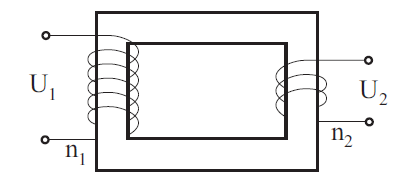
\includegraphics[width=0.5\textwidth]{abb1}
	\end{center}
	\caption{Umspanner, Transformator, $n_i$ Windungszahlen der jeweiligen Spule}
	\label{fig:abb1}
\end{figure}

Die Netzspannung

\begin{equation}
	U_1 = U_0 \, \sin{(\omega t)}
\end{equation}

erzeugt einen Strom $I_1$(t) im Primärkreis. Dieser Strom bewirkt einen magnetischen Fluss $\phi$(t)
in der Spule. Die Flussänderung induziert eine Spannung $U_L$ in der Spule mit der Windungszahl
$n$.

\begin{equation}
	U_L = -n_1 \der{\phi}{t}
\end{equation}

Für den Primärkreis gilt also:

\begin{equation}
	U_1 + U_L = 0
\end{equation}

\begin{equation}
	U_0 \, \sin{(\omega t)} = n_1 \der{\phi}{t}
	\label{eq:aleksey}
\end{equation}

Das ergibt den Fluss:

\begin{equation}
	\phi (t) = \frac{U_0}{n_1 \omega} \, \sin(\omega t - \pi / 2)
\end{equation}

Damit ist der magnetische Fluss $\phi(t)$ durch die Netzspannung $U_1(t)$ vorgegeben.

\newpage

\subsubsection{Leerlauf}

$I_2$ = 0. Die Flussänderung induziert in der Sekundärspule eine Spannung $U_2$:

\begin{align*}
	U_2 & = - n_2 \der{\phi}{t} = -\frac{n_2}{n_1} U_0 \; \sin{(\omega t)}
\end{align*}
\begin{align}
	U_2 = -\frac{n_2}{n_1} U_1(t) \qquad \qquad
\end{align}

Das Verhältnis der Spannungen ist somit durch die Windungszahlen gegeben. Der Strom im
Primärkreis wird nur durch das Magnetisierungsverhalten des Eisens festgelegt.

\begin{equation}
	\phi = B A = \mu \mu_0 H A = \mu \mu_0 \frac{A}{l} n_1 l_1
\end{equation}

Bei linearer Magnetisierungsabhängigkeit des verwendeten Eisens (\autoref{fig:abb2}) ist der Strom dem
von ihm hervorgerufenen Fluss proportional. Es wird daher auch die Stromwelle der angelegten
Spannung um $\pi / 2$ nacheilen.

Die elektrische Leistung eines Gerätes ist durch das Produkt von Spannung und Strom gegeben.
Die Leistung $N$ an der Primärspule in Abhängigkeit von der Zeit bei Nacheilen des Stromes
gegenüber der Spannung um $\pi / 2$ zeigt \autoref{fig:abb3}. Man erkennt, dass das Vorzeichen der Leistung
wechselt. Die aufgenommene Arbeit wird also stets wieder an das Netz zurückgegeben. Man
nennt das Produkt $U_1 I_b$ im Falle einer Phasenverschiebung von $\pi / 2$ Blindleistung $Q_1$. Der aufgenommene
Blindstrom $I_b$ wird Magnetisierungsstrom genannt.

\begin{minipage}{\textwidth}
	\begin{minipage}[t]{0.5\textwidth}
		\centering
		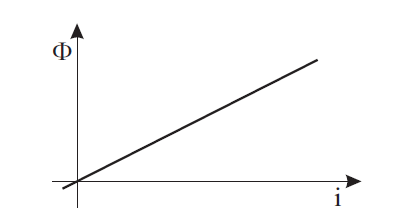
\includegraphics[width=\textwidth]{abb2}
		\captionbelowof{figure}{Eisen mit gerader Magnetisierungskurve}
		\label{fig:abb2}
	\end{minipage}
	\vspace{2mm}
	\begin{minipage}[t]{0.50\textwidth}
		\centering
		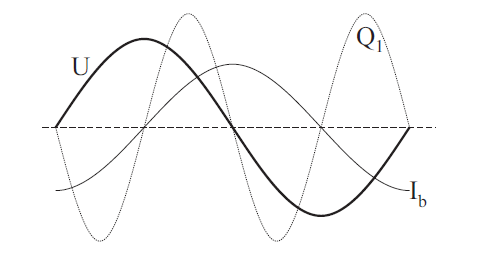
\includegraphics[width=\textwidth]{abb3}
		\captionof{figure}{Blindleistung $Q_1 = UI_b$}
		\label{fig:abb3}
	\end{minipage}
	\vspace{1em}
\end{minipage}

Für den Fall, dass die Magnetisierungskurve $\phi = \phi (t)$ eine Hysterese aufweist, entsteht der
Stromverlauf aus \autoref{fig:abb4}. Dem Netz wird in diesem Fall Leistung entzogen.

\begin{figure}[H]
	\begin{center}
		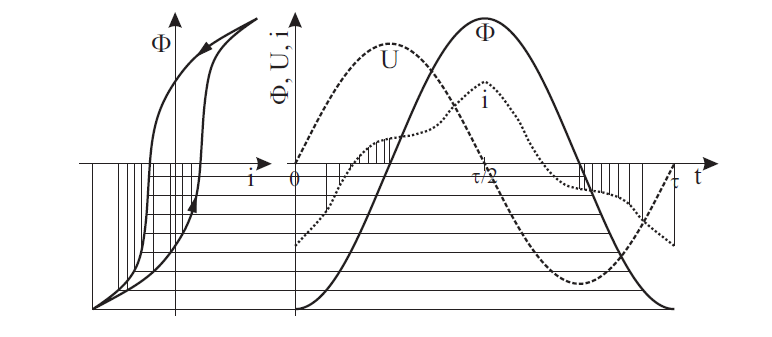
\includegraphics[width=0.8\textwidth]{abb4}
	\end{center}
	\caption{Spannung $U$, magnetischer Fluss $\phi$ und Strom $i$ bei Hysterese.}
	\label{fig:abb4}
\end{figure}

\subsubsection{Belastung}

Wird an die Sekundärspule ein Ohm’scher Widerstand $R$ angeschlossen, so fließt auch durch
die Sekundärspule ein Strom $I_2$

\begin{equation}
	I_2 = \frac{U_2}{R} = -\frac{n_2}{n_1}\frac{1}{R} \,U_0\, \sin{(\omega t)}
\end{equation}

Jede stromdurchflossene Spule erzeugt ein Magnetfeld. Die stromdurchflossene Sekundärspule
erzeugt einen von $I_2$ unabhängigen Zusatzfluss $\phi_2$, der durch die Magnetisierungskurve bestimmt
ist. Da der Fluss aber durch Gl. (5) wegen der eingeprägten Netzspannung festgelegt ist, muss
$\phi_2$ kompensiert werden:

\begin{equation}
	\phi_2 + \phi_1 = 0
\end{equation}

Diese Kompensation erfolgt durch einen in der Primärspule erzeugten Fluss $\phi_1$, der durch einen
Zusatzstrom $I_{1_z}$ zustande kommt. Mit

\begin{equation}
	\phi_2 = \phi \, \phi_0 \frac{A}{l}n_2 l_2
\end{equation}

und

\begin{equation}
	\phi_1 = \phi\, \phi_0 \frac{A}{l}n_1 l_{1_z}
\end{equation}

ergibt sich $I_{1_z}$ aus der Bedingung Gl. (9)

\begin{equation}
	I_{1_z} = - \frac{n_2}{n_1} I_2
\end{equation}

und wegen Gl. (8):

\begin{equation}
	I_{1_z} = \left(\frac{n_2}{n_1}\right)^2 \frac{1}{R} \, U_1
\end{equation}

Der primäre Zusatzstrom ist bei der angenommenen rein Ohm’schen Belastung in Phase mit
der Netzspannung $U_1$. Der durch rein Ohm’sche Belastung der Sekundärseite bewirkte primäre
Zusatzstrom $I_{1_z}$ verursacht eine Wirkleistungsaufnahme. Das Produkt der $U_1$ - und $I_{1_z}$ - Wellen ist
nämlich stets positiv. Selbstverständlich existieren die beiden Ströme $I_b$ und $I_{1_z}$ nicht getrennt.
Sie setzen sich zu einem Netzstrom $I_1$ zusammen. Dies geschieht, indem man die zu gleichen
Zeiten gehörenden Momentanwerte addiert.

Eine Sinuswelle entsteht z.B. durch einen mit der Winkelgeschwindigkeit $\omega$ rotierenden Zeiger,
wenn man die Spitze des Zeigers in Abhängigkeit vom Winkel $\omega t$ beobachtet (\autoref{fig:abb5}).

\begin{figure}[H]
	\begin{center}
		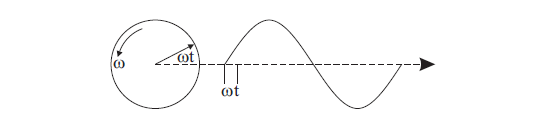
\includegraphics[width=0.8\textwidth]{abb5}
	\end{center}
	\caption{Zeigerdiagramm und Sinusschwingung}
	\label{fig:abb5}
\end{figure}

Addiert man die Momentanwerte zweier mit gleicher Winkelgeschwindigkeit rotierender Größen,
welche gegeneinander eine Phasenverschiebung haben, so setzen sich die Zeiger geometrisch zusammen
(\autoref{fig:abb6}). Für den belasteten Transformator zeigt \autoref{fig:abb7} die Lage der Zeiger. Die
Phasenverschiebung $\phi$ zwischen dem Gesamtstrom $I_1$ (auch Scheinstrom genannt) und der Netzspannung
ist nach \autoref{fig:abb7} gegeben durch:

\begin{equation}
	\tan(\phi) = \frac{I_b}{I_{1_z}} \qquad \cos(\phi) = \frac{I_{1_z}}{I_1} \qquad \sin(\phi) = \frac{I_b}{I_1}
\end{equation}

\begin{minipage}{\textwidth}
	\begin{minipage}[t]{0.6\textwidth}
		\centering
		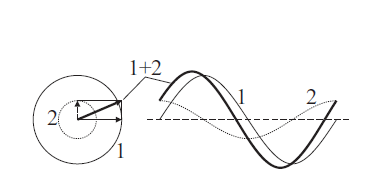
\includegraphics[width=\textwidth]{abb6}
		\captionbelowof{figure}{Addition zweier Sinusschwingungen}
		\label{fig:abb6}
	\end{minipage}
	\vspace{2mm}
	\begin{minipage}[t]{0.4\textwidth}
		\centering
		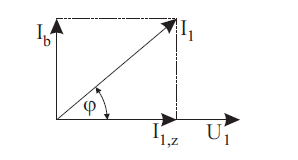
\includegraphics[width=\textwidth]{abb7}
		\captionof{figure}{Zeigerdiagramm im belasteten Transformator}
		\label{fig:abb7}
	\end{minipage}
	\vspace{1em}
\end{minipage}

Da die Multiplikation der Zähler und Nenner mit $U_1$ an den Verhältnissen Gl. (14) nichts ändert,
gilt auch:

\begin{equation}
	\tan(\phi) = \frac{Q_1}{P_1} \qquad \cos(\phi) = \frac{P_1}{S_1} \qquad \sin(\phi) = \frac{Q_1}{S_1}
\end{equation}

Dabei ist $I_{1_z} U_1$ die Wirkleistung $P_1$, $I_b U_1$ die Blindleistung $Q_1$ und $I_1 U_1$ die Scheinleistung $S_1$.

Bei verlustlosem Transformator muss, damit der Energieerhaltungssatz gewahrt
bleibt, die zugeführte Wirkleistung gleich der sekundär abgegebenen
Wirkleistung sein:

\begin{equation}
	I_{1_z} U_1 = P_1 = P_2 = U_2 I_2
\end{equation}

\subsubsection{Verluste im Transformator}

Die Spulen des Transformators haben endliche Widerstände: $R_{Sp1}$ und $R_{Sp2}$. Die an ihnen auftretende
Wirkleistung

\begin{equation}
	P_{Cu1} = R_{Sp1} \, I_1^2 \qquad \qquad P_{Cu2} = R_{Sp2} \, I_2^2
\end{equation}

wird als Wärme frei. Ihre Summe $P_{Cu}$ bezeichnet man als Kupferverluste des Transformators.

\begin{equation}
	P_{Cu} = P_{Cu1} + P_{Cu2}
\end{equation}

Außer den Kupferverlusten treten im Transformator auch sogenannte Eisenverluste auf. Sie
setzen sich aus den Wirbelstromverlusten und den Hystereseverlusten zusammen. Die Wirbelstromverluste
entstehen durch die elektrische Leitfähigkeit des Eisens. Der Wechselfluss induziert
auch im Eisen Spannungen, die sogenannte Wirbelströme hervorrufen, und eine Erwärmung des
Eisens bewirken. Durch Unterteilung des Eisenkerns in dünne, gegenseitig isolierte Bleche, kann
man das Auftreten von gut leitenden Stromkreisen im Eisen weitgehend verhindern.

Die Hystereseverluste entstehen durch die Abweichung der Eisenmagnetisierung von der Idealform
in \autoref{fig:abb2}. Es zeigt sich nämlich, dass nach Zurückgehen des Stromes auf den Wert Null
Restmagnetismus (Remanenz) vorhanden ist (\autoref{fig:abb8}). Wird nun in umgekehrter Richtung ein
Magnetfeld aufgebracht, so muss erst Energie aufgewendet werden, um das Restfeld abzubauen.
Infolge der Transformatorverluste sinkt die Spannung $U_2$ an der Sekundärspule.

\begin{figure}[H]
	\begin{center}
		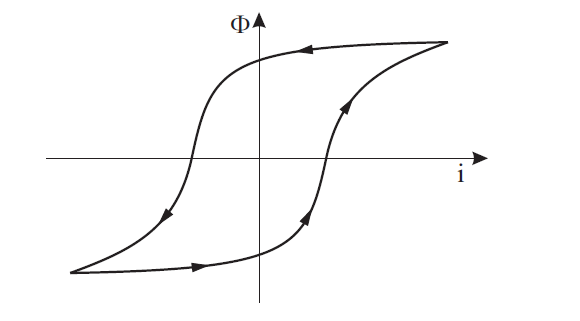
\includegraphics[width=0.5\textwidth]{abb8}
	\end{center}
	\caption{Hystereseschleife}
	\label{fig:abb8}
\end{figure}



\newpage

\section{Versuchsanordnung \cite{vorlagetrafo}}\label{sec:Versuchsanordnung}

Ablesungen in Abhängigkeit vom Belastungswiderstand (Last) nach \autoref{fig:abb9} erlauben es, folgende
Größen zu berechnen:

\begin{itemize}

	\item Abgegebene Wirkleistung: $P_2 = U_R\,I_2$

	\item Aufgenommene Scheinleistung: $S_1 = U_1\,I_1$

	\item Phasenverschiebung an der Primärseite: $\cos{(\phi)}$ = $P_1 / S_1, \phi = $ arccos($P_1 / S_1$)

	\item Primärer Wirkstrom: $I_{1_z} = I_1 \cos{(\phi)}$

	\item Primärer Blindstrom: $I_b = I_1 \sin{(\phi)} = I_1 \sqrt{1 - \cos^2(\phi)}$

	\item Primäre Blindleistung: $Q_1 = I_b U_1$

	\item Verlustleistung: $\Delta P = P_1 - P_2$ als Differenz der zugeführten und der abgegebenen elektrischen Leistung.

	\item Wirkungsgrad: $\eta = N_2 / N_{1_{\omega}} \cdot 100\%$ welcher angibt, wie viel Prozent der zugeführten Leistung als elektrische Energie sekundär zur Verfügung steht.

	\item Kupferverluste:

	      \begin{itemize}

		      \item Primär: $P_{Cu1} = I_1^2 \, R_{Sp1}$

		      \item Sekundär: $P_{Cu2} = I_2^2 \, R_{Sp2}$

		      \item Insgesamt: $P_{Cu} = P_{Cu1} + P_{Cu2}$

	      \end{itemize}

	\item Eisenverluste: $P_{Fe} = \Delta P - P_{Cu}$

\end{itemize}

\begin{figure}[H]
	\begin{center}
		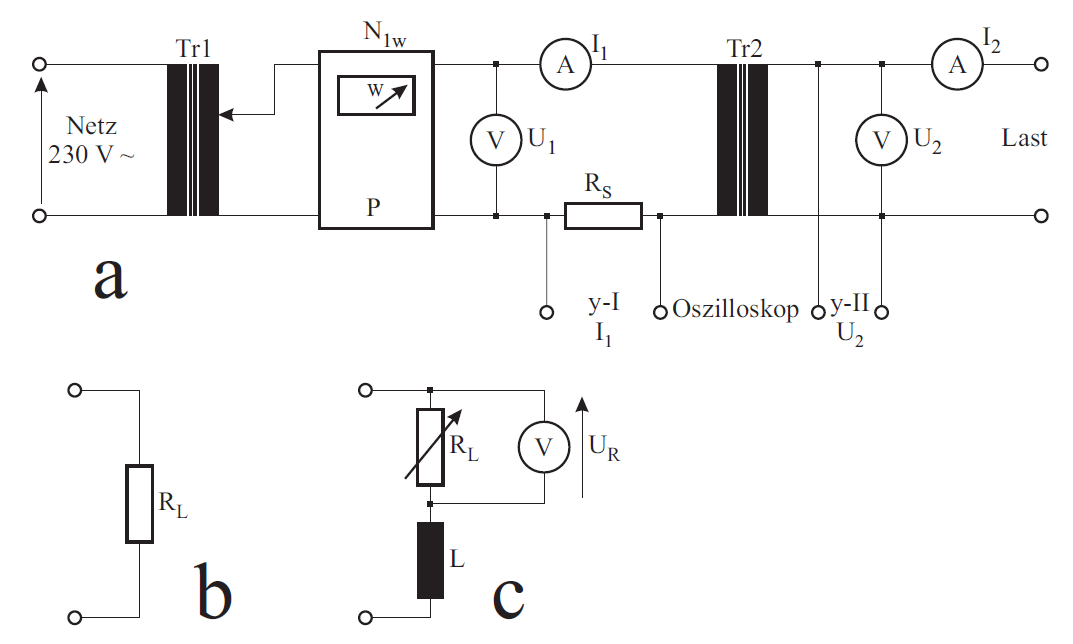
\includegraphics[width=\textwidth]{abb9}
	\end{center}
	\caption{Messanordnung zur Untersuchung des Transformators Tr2 für $a$) Leerlauf, \\
		$b$) ohm’sche Last, $c$) ohm’sche und induktive Last in Serie. \\
		Tr1 $\dots$ Regeltrenntrafo \\
		Tr2 $\dots$ Messtrafo \\
		$R_S \dots$ Shunt (ca. 0.5 $\Omega$) \\
		$R_L \dots$ Lastwiderstand \\
		$I_1 \dots$ Primärstrom \\
		$U_1 \dots$ Primärspannung \\
		$I_2 \dots$ Sekundärstrom \\
		$U_2 \dots$ Sekundärspannung \\
		$L \dots$ Spule \\
		$C \dots$ Kondensator \\
		$U_R \dots$ Spannungsabfall an $R_L$ \\
		$P_1 \dots$ primäre Wirkleistung}
	\label{fig:abb9}
\end{figure}


\newpage

\section{Geräteliste}

\noindent Für die Messungen wurden folgende Geräte vom Versuchsaufbau Transformator 1 verwendet:

\captionof{table}{Verwendete Geräte }
\begin{center}
	\begin{tabular}{|c|c|c|c|} \hline
		\textbf{Gerät}                               & \textbf{Typ}       & \textbf{Hersteller} & \textbf{Unsicherheit}    \\ \hline

		Transformator 1                              & Prim SI 6.3A1      &                     &                          \\ \hline
		Transformator 2                              & 163/JFR/14         &                     &                          \\ \hline
		Digital Multimeter                           & 531832             & LeyBold             & $\pm$ \SI{0.1}{\watt}    \\ \hline
		Oszilloskop                                  & DS1052E            & RiGol               & $\pm$ \SI{1}{\percent}   \\ \hline
		Computerprogramm                             & Ultrascope         &                     &                          \\ \hline
		Shunt                                        & 163/SFR/14         &                     &                          \\ \hline
		Spule                                        & \SI{2.58}{\ohm}    &                     &                          \\ \hline
		regelbarer Widerstand                        & PF80/3.3A  VII/695 & Western Germany     &                          \\ \hline
		Voltmeter Bereich (\SIrange{30}{240}{\volt}) & VII/1111/3         &                     & $\pm$ \SI{0.5}{\percent} \\ \hline
		Voltmeter Bereich (6-60 V)                   & VII/1121/2         &                     & $\pm$ \SI{0.5}{\percent} \\ \hline
		Voltmeter Bereich (6-60 V)                   & VII/1121/3         &                     & $\pm$ \SI{0.5}{\percent} \\ \hline
		Amperemeter Bereich (0.24-6 A)               & VII/1106/9         &                     & $\pm$ \SI{1.5}{\percent} \\ \hline
		Amperemeter Bereich (1.2-6 A)                & VII/1130/          &                     & $\pm$ \SI{0.5}{\percent} \\ \hline
		Probe für Oszilloskop                        & \num{20141071}     & RS                  &                          \\ \hline
		Probe für Oszilloskop                        & 20140783           & RS                  &                          \\ \hline
		Kabel                                        & Bananenstecker     &                     &                          \\ \hline
	\end{tabular}
	\label{tab:material}
\end{center}

\newpage

\section{Versuchsdurchführung \& Messergebnisse}\label{sec:Versuchsdurchführung}

\subsection{Leerlauf}

Zunächst wird der Versuch nach der Skizze in
\autoref{fig:abb9} a) aufgebaut. Um einen besseren
Überblick über die Schaltung zu behalten, wird der
Weg vom Trafo bis zur Last, die in diesem Aufbau
noch nicht vorhanden ist, mit gelben Kabeln und der
Rückweg mit grünen Kabeln markiert. Die parallel
geschalteten Voltmeter sind mit blauen und die
Proben des Oszilloskops mit roten und schwarzen
Kabeln mit dem Stromkreis verbunden. Der komplette
Versuchsaufbau ist in \autoref{fig:leerlauf}
ersichtlich.

Bei den Vollmetern ist dabei zu beachten, dass sich jenes, welches für die
größeren Spannungen ausgelegt ist, vor dem Transformator befindet, um
sicherzustellen, dass das andere Voltmeter nicht überlastet wird. Bei den
Amperemetern wird jenes mit dem geringeren Messbereich vor den Transformator
geschlossen, da hier aufgrund der deutlich höheren Spannung niedrigere Ströme
vorliegen. Auch ist bei den Messgeräten grundsätzlich immer der größte
Messbereich zu verwenden und erst nach Beurteilung des Zeigerausschlags auf den
nächst niedrigeren Bereich zu wechseln, um sicherzustellen, dass kein Messgerät
überlastet wird.

\begin{figure}[H]
	\begin{center}
		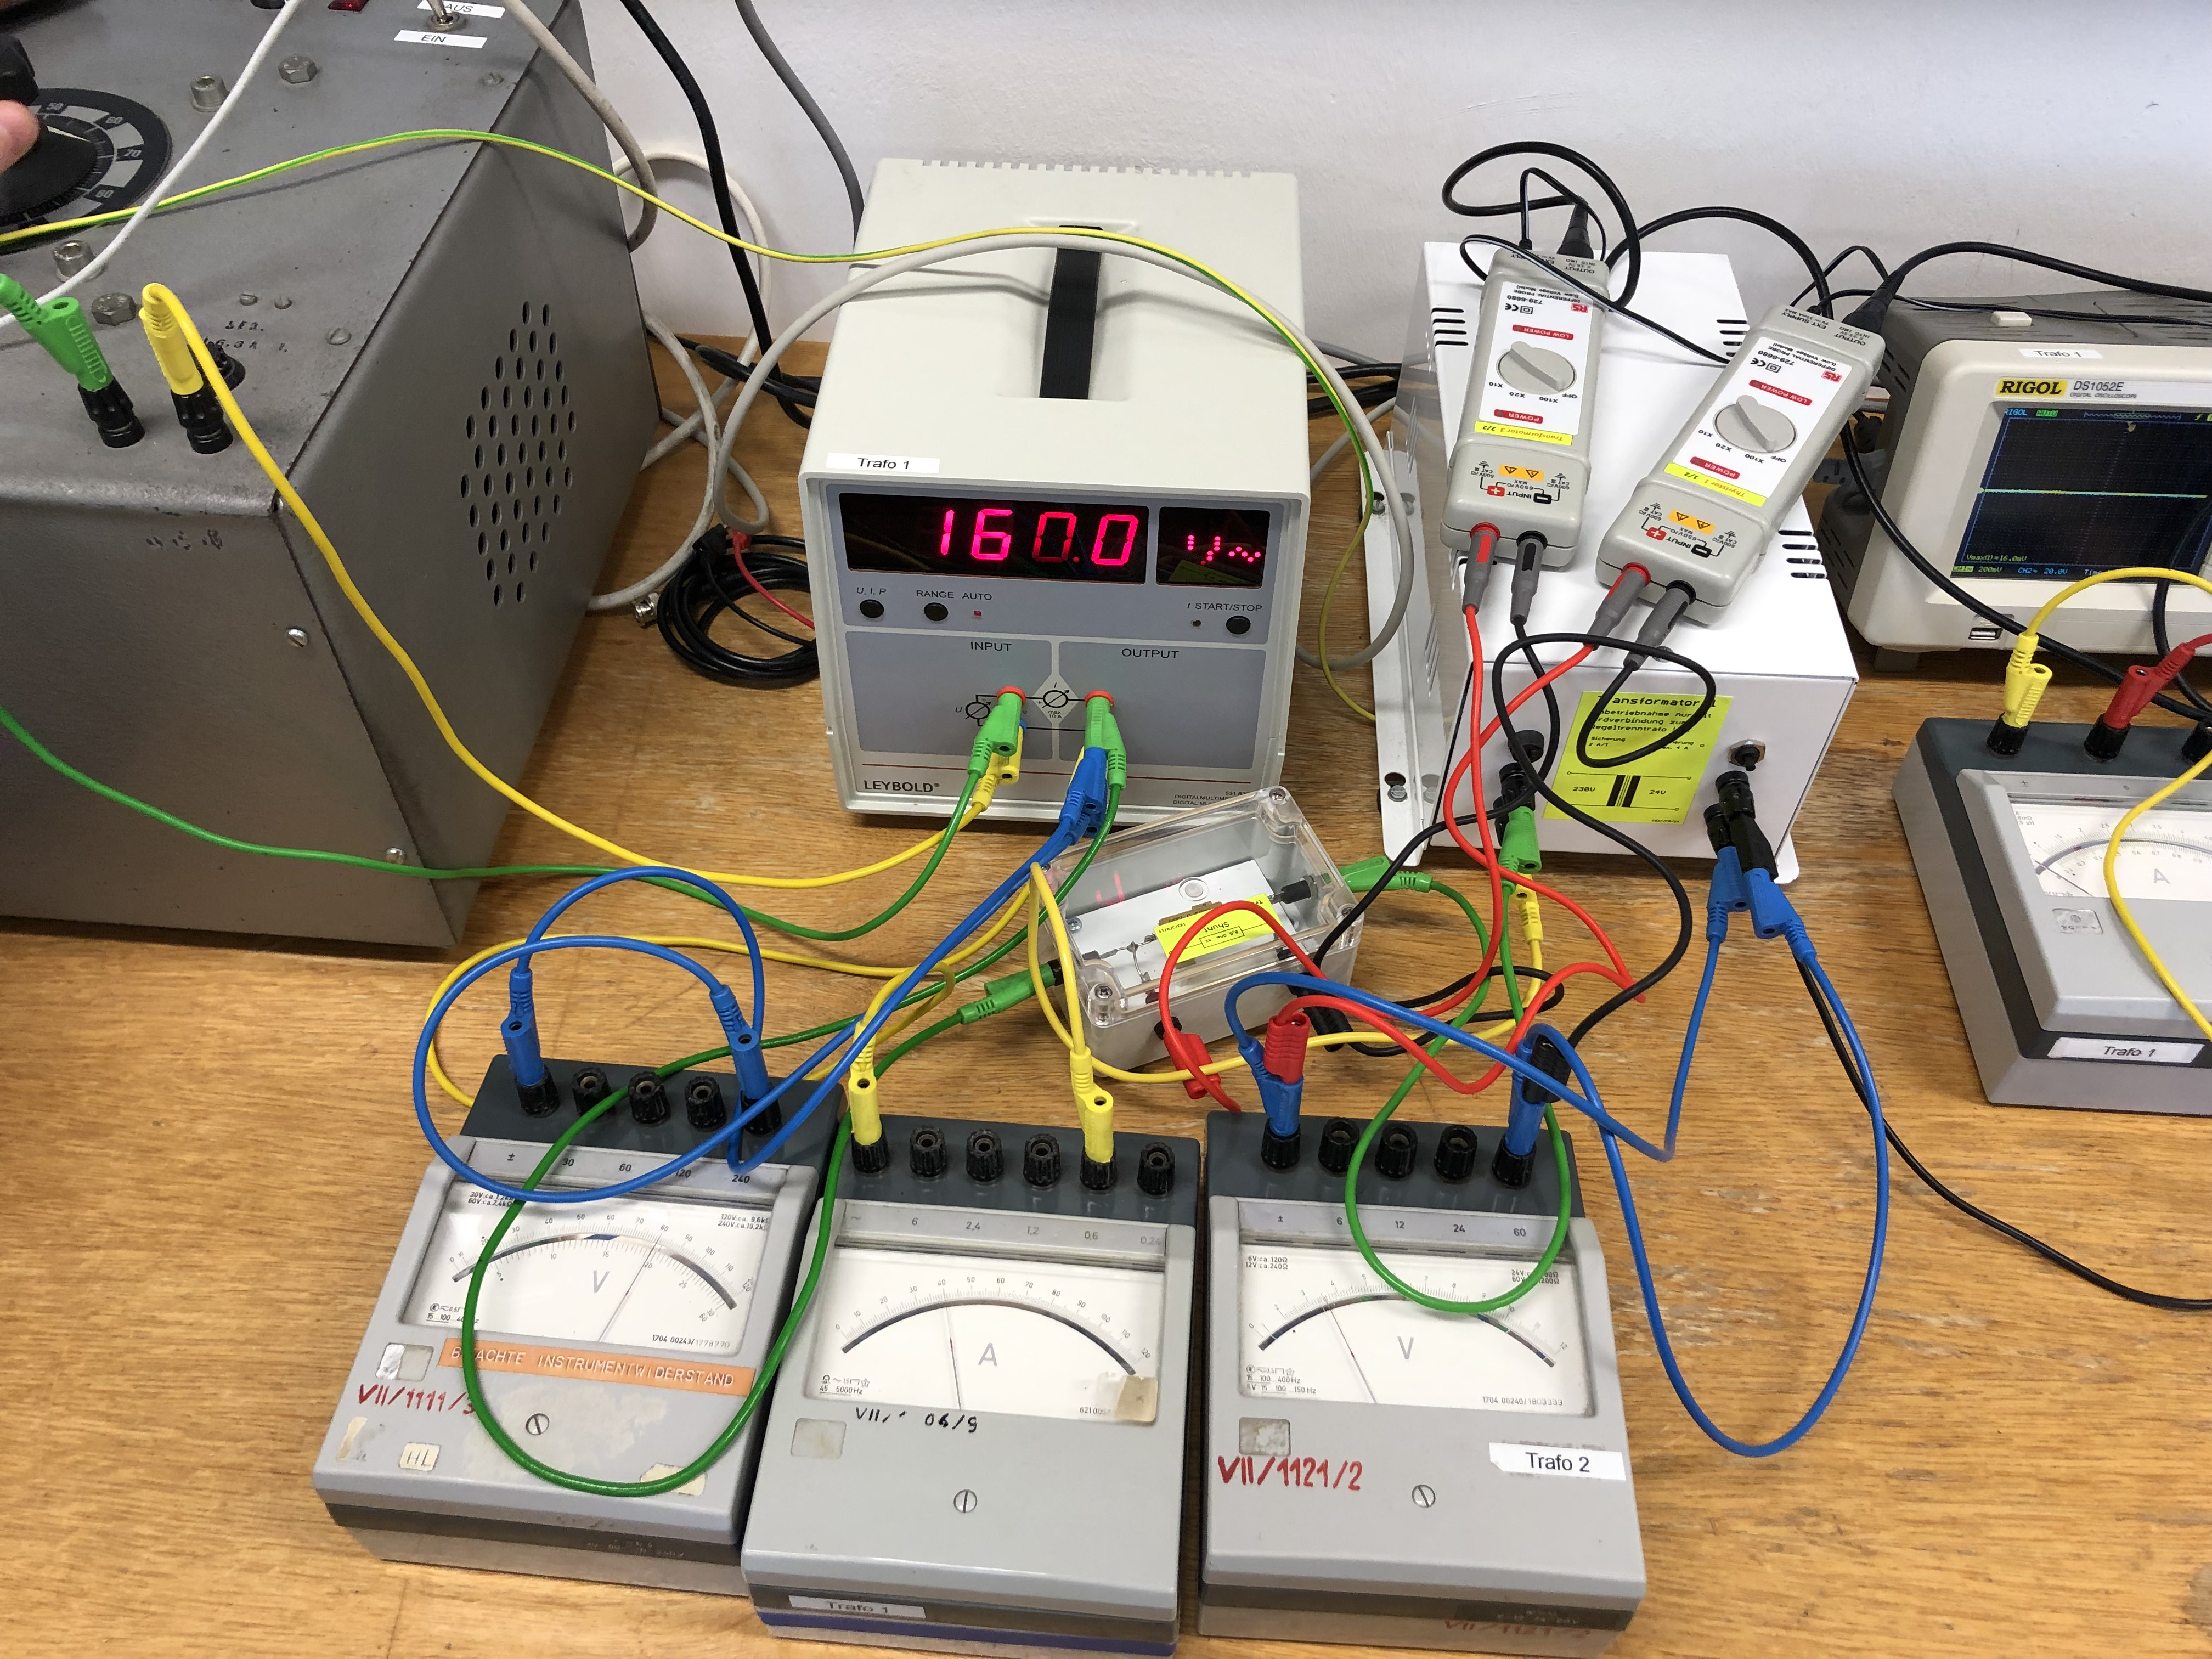
\includegraphics[width=0.7\textwidth]{leerlauf}
	\end{center}
	\caption{Versuchsaufbau für den Leerlauf}
	\label{fig:leerlauf}
\end{figure}

Nun werden die geforderten Ströme und Spannungen von den Ampere- und
Voltmetern, sowie die Leistung der Primärspannung am digitalen Multimeter
abgelesen und in folgender \autoref{tab:daten_versuch1} aufgelistet. Die
Unsicherheit der entsprechenden Werte setzt sich dabei aus der Unsicherheit des
Geräts, die bereits in \autoref{tab:material} aufgelistet ist, sowie der
Ableseunsicherheit der analogen Messgeräte, die als ein halber Skalenstrich
angenommen wurde, zusammen.


\begin{table}[H]
	\caption{Gemessene Daten der a Schaltung. Folgende Werte beziehen sich auf
		\autoref{fig:abb9} in Schaltung a. Die Unsicherheit setzt sich dabei aus
		der Unsicherheit des Geräts und der Ableseunsicherheit zusammen, was im
		folgenden ersichtlich ist.\\
		$P_1$ \dots primäre Wirkleistung, $\Delta P_1 =$ \SI{0.1}{W} \\
		$U$ \dots VARIAC eingestellte Netzspannung, $\Delta U =$ \SI{0.1}{V}\\
		$U_1$ \dots  Primärspannung, $\Delta U_1 =$ 1,2 + 1,0 = \SI{3}{V} \\
		$I_1$ \dots Primärstrom, $\Delta I_1 =$ 0,009 + 0,0025 = \SI{0.012}{A} \\
		$U_2$ \dots Sekundärspannung, $\Delta U_2 =$ 0,12 + 0,10 = \SI{0.3}{V}  \\
	}
	\label{tab:daten_versuch1}
	\begin{center}
		\begin{tabular}{lrrrrrr}
	\toprule
	{} & $P_1$ / \si{\watt} & $U$ / \si{\volt} & $U_1$ / \si{\volt} & $I_1$ / \si{\ampere} & $U_2$ / \si{\volt} \\
	\midrule
	0  & 7.4                & 160.0            & 161.0              & 0.200                & 14.4               \\
	\bottomrule
\end{tabular}

	\end{center}
\end{table}



\subsection{Ohm´sche Last}

Nun wird, wie in der Skizze in \autoref{fig:abb9} b) dem Aufbau ein Widerstand hinzugefügt, wodurch sich folgender Aufbau ergibt.

\begin{figure}[H]
	\begin{center}
		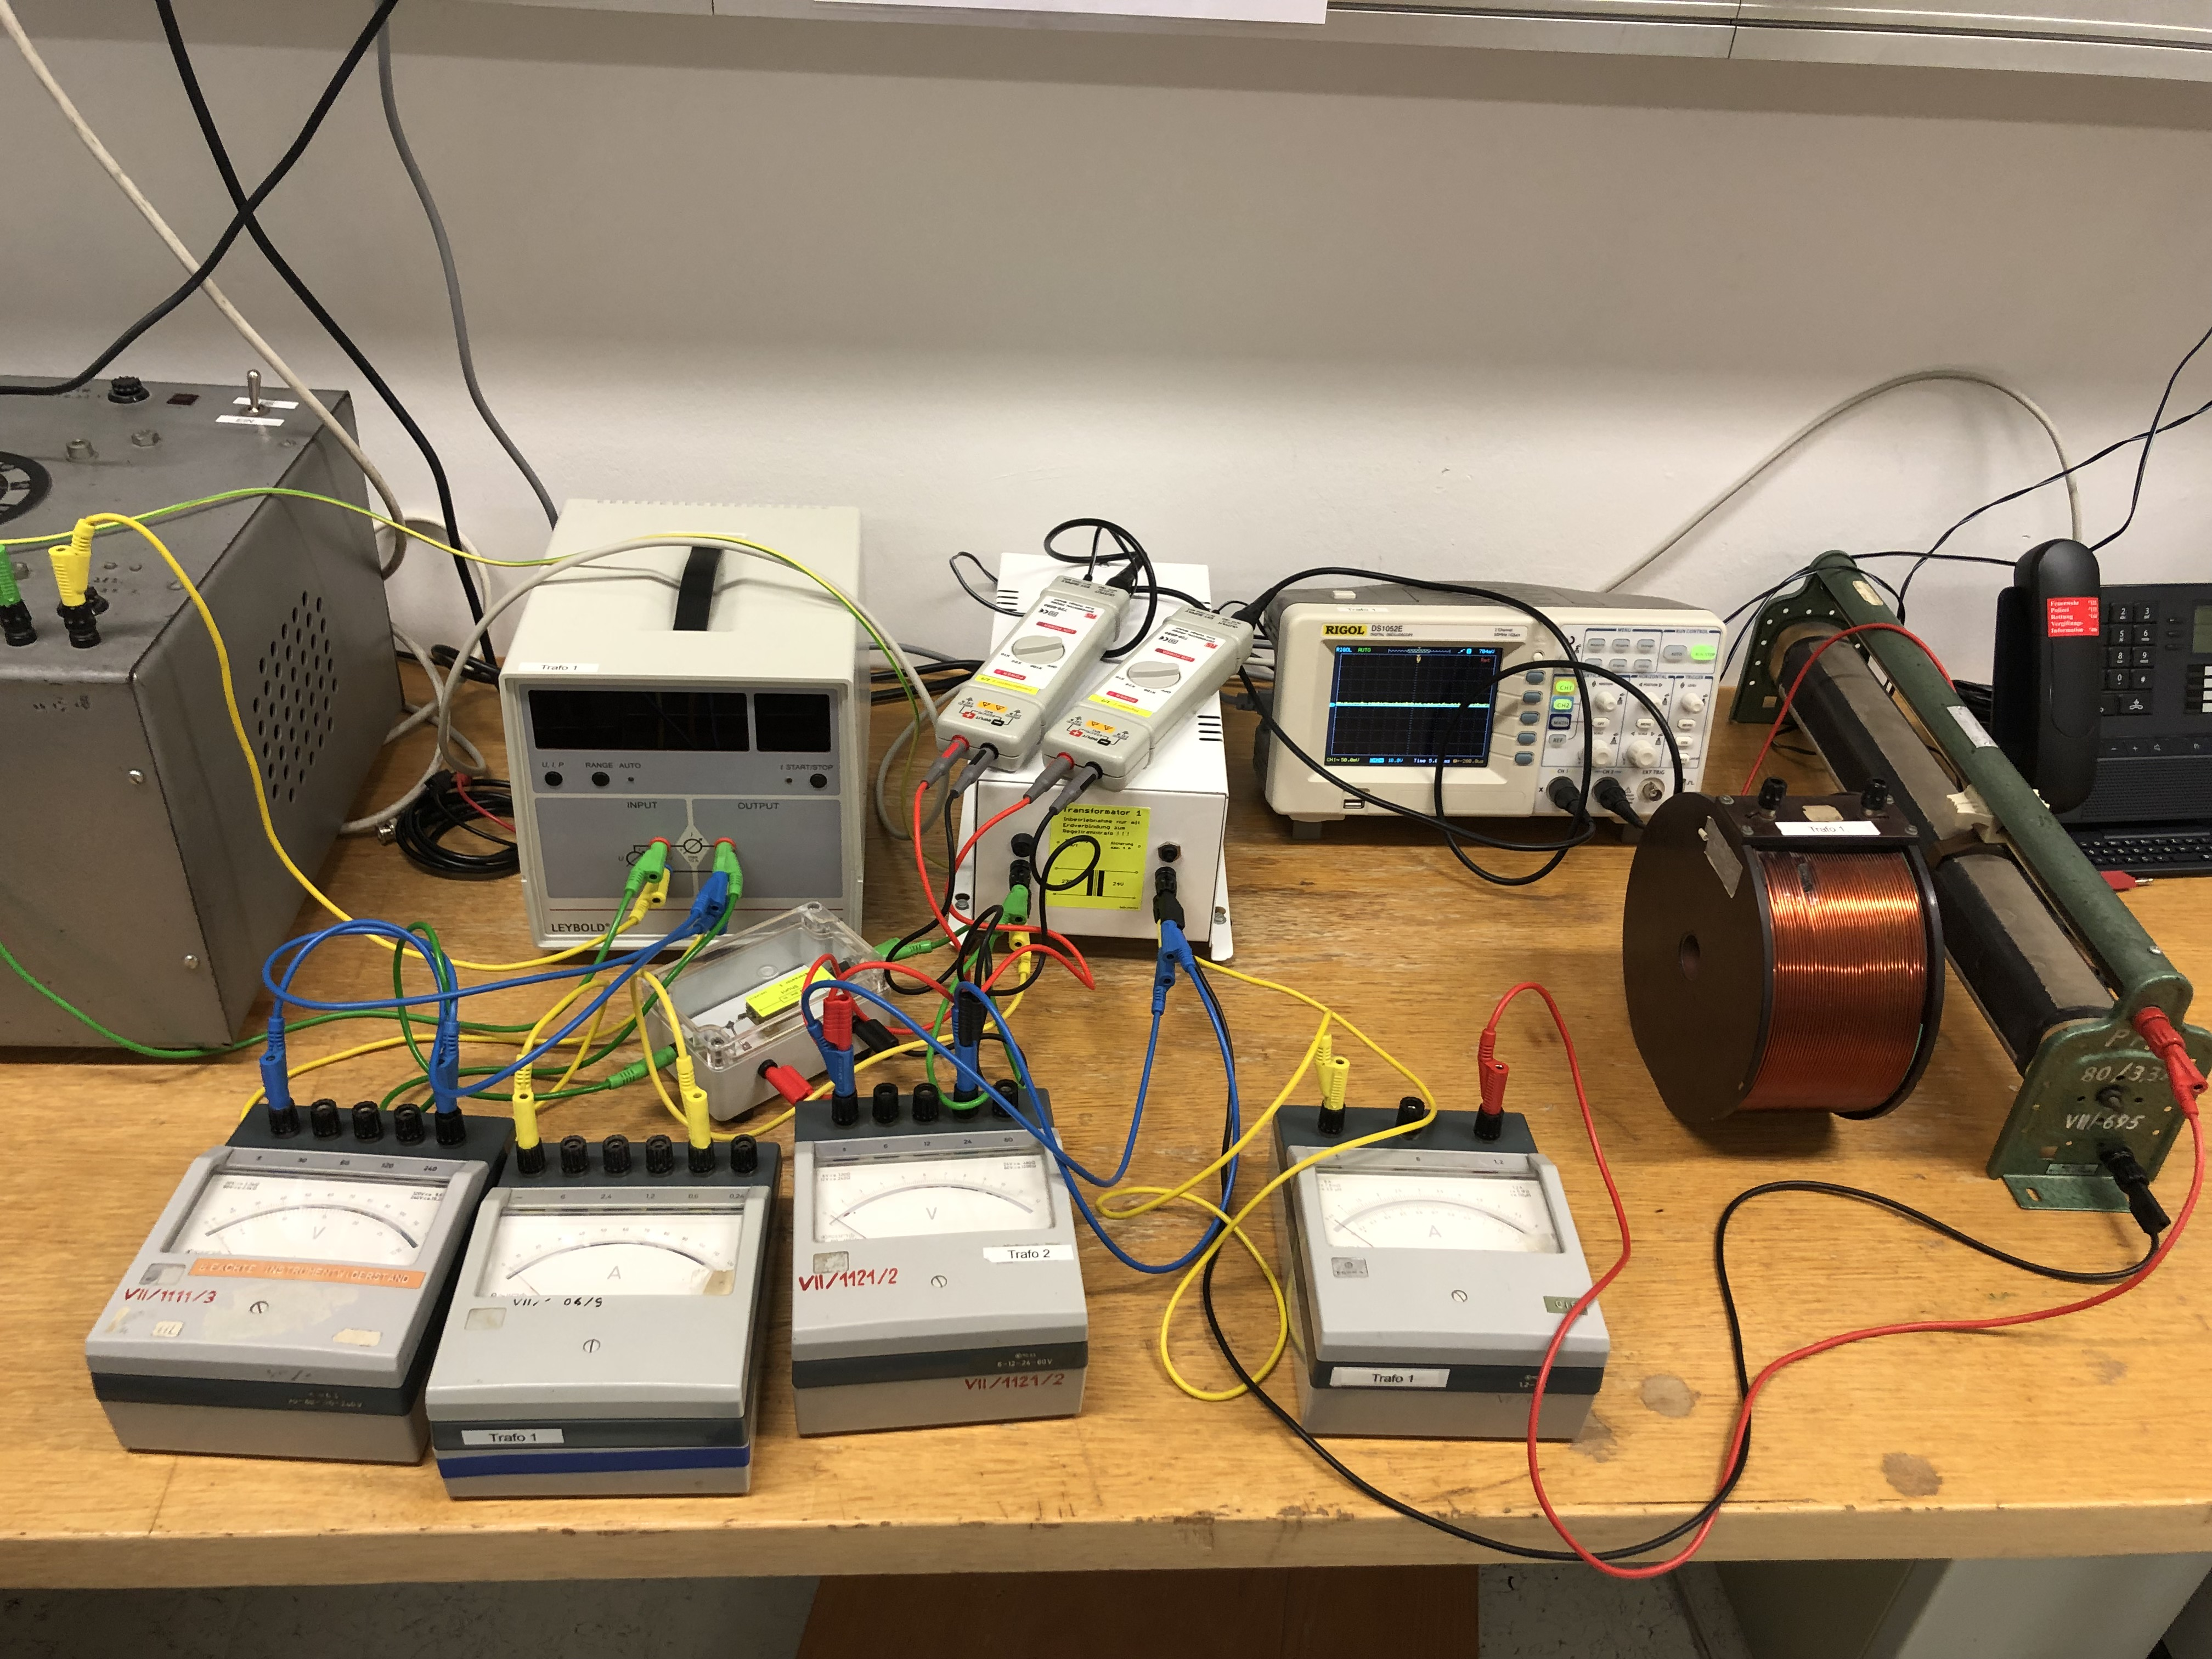
\includegraphics[width=0.7\textwidth]{widerstand}
	\end{center}
	\caption{Versuchsaufbau für die Ohm´sche Last}
	\label{fig:widerstand}
\end{figure}

Die abgelesenen Werte der Geräte sind in folgender \autoref{tab:daten_versuch2} aufgelistet:

\begin{table}[H]
	\caption{Gemessene Daten der b Schaltung. Folgende Werte beziehen sich auf \autoref{fig:abb9} in Schaltung b. Die Unsicherheit setzt sich dabei aus der Unsicherheit des Geräts und der Ableseunsicherheit zusammen, was im folgenden ersichtlich ist.\\
		$P_1$ \dots primäre Wirkleistung, $\Delta P_1 =$ \SI{0.1}{W}\\
		$U_1$ \dots  Primärspannung, $\Delta U_1 =$ 1,2 + 1,0 = \SI{3}{V} \\
		$I_1$ \dots Primärstrom, $\Delta I_1 =$ 0,009 + 0,0025 = \SI{0.012}{A} \\
		$U_2$ \dots Sekundärspannung, $\Delta U_2 =$ 0,12 + 0,10 = \SI{0.3}{V}  \\
		$I_2$ \dots Sekundärstrom, $\Delta I_2 =$ 0,006 + 0,005 = \SI{0.011}{A} \\
	}
	\label{tab:daten_versuch2}
	\begin{center}
		\begin{tabular}{lrrrrrr}
	\toprule
	{} & $P_1$ / \si{\watt} & $U_1$ / \si{\volt} & $I_1$ / \si{\ampere} & $U_2$ / \si{\volt} & $I_2$ / \si{\ampere} \\
	\midrule
	0  & 25.2               & 162.0              & 0.255                & 16.1               & 1.010                \\
	\bottomrule
\end{tabular}

	\end{center}
\end{table}


\subsection{Ohm´sch-induktive Last}

Zuletzt wird dem Aufbau noch eine Spule, sowie ein Voltmeter hinzugefügt, wie
in der Skizze in \autoref{fig:abb9} c) ersichtlich. Unter Beibehaltung des
zuvor erklärten Farbschemas der Kabel ergibt sich nun folgender Aufbau.

\begin{figure}[H]
	\begin{center}
		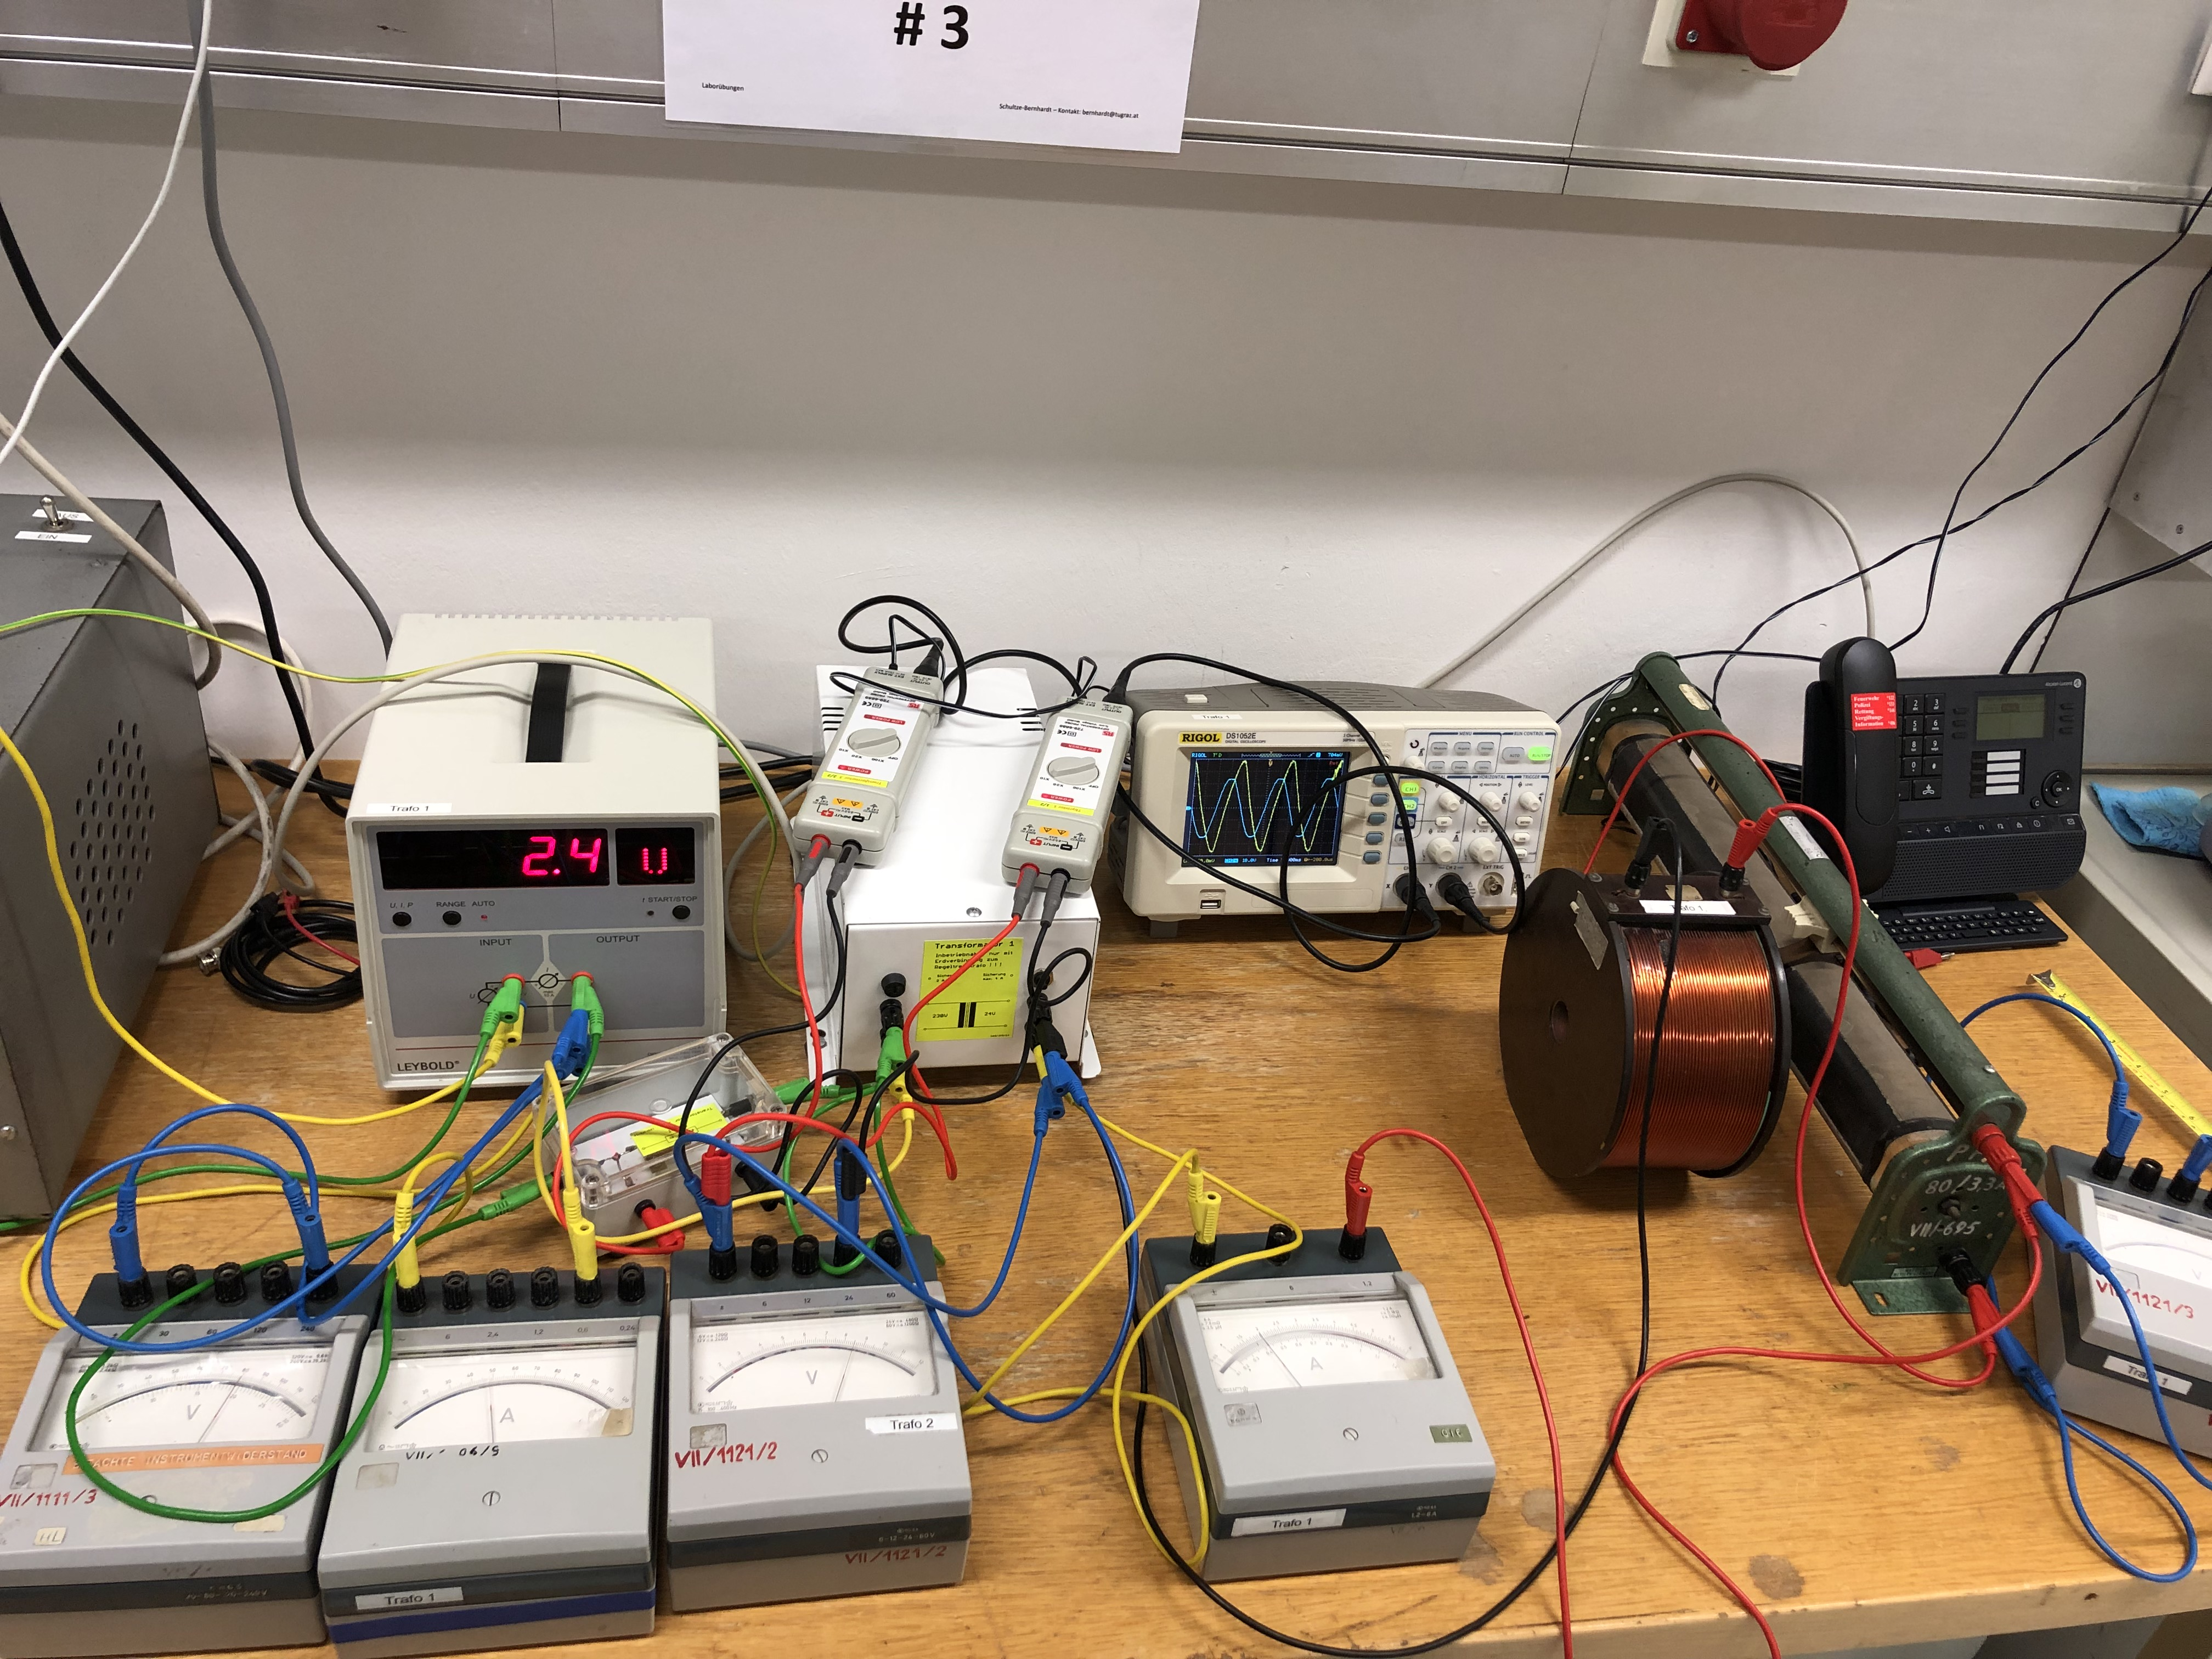
\includegraphics[width=0.7\textwidth]{spule}
	\end{center}
	\caption{Versuchsaufbau für die Ohm´sch-induktive Last}
	\label{fig:spule}
\end{figure}

Im Zuge dieses Versuchs, soll der Widerstand zwischen 0 und 45 $\Omega$
variiert und ca. 20 Messungen durchgeführt werden. Dazu wird zunächst die
Position des Reglers gesucht, bei dem der Widerstand ca. 45 $\Omega$ beträgt,
sowie jene Position, bei der das entsprechende Voltmeter den gierigsten Wert
der Spannung der noch aufgelöst werden kann, verzeichnet. Da die Differenz
dieser beiden Punkte \SI{24.0(5)}{\cm} entspricht,
wurde entschieden den Regler immer um ca. \SI{1}{\cm} zu verschieben.

Alle abgelesenen Werte, sowie deren Unsicherheit, sind in nachfolgender
\autoref{tab:daten_versuch3} und \autoref{tab:daten_versuch3_2} aufgelistet:

%{tab:daten_versuch3}
\begin{table}[H]
	\caption{
		Erste Tabelle der gemessene Daten der c Schaltung. Folgende Werte beziehen
		sich auf \autoref{fig:abb9} in Schaltung c. Die Unsicherheit setzt sich
		dabei aus der Unsicherheit des Geräts und der Ableseunsicherheit zusammen,
		was im folgender Tabelle ersichtlich ist.\\
		$P_1$ \dots primäre Wirkleistung \\
		$U$ \dots VARIAC eingestellte Netzspannung \\
		$U_1$ \dots  Primärspannung \\
		$I_1$ \dots Primärstrom \\
		$\Delta$ \dots entsprechende Unsicherheit
	}
	\label{tab:daten_versuch3}
	\begin{center}
		\begin{tabular}{lrrrrrrrr}
	\toprule
	{} & $P_1$ / \si{\watt} & $\Delta P_1$ / \si{\watt} & $U$ / \si{\volt} & $\Delta U$ / \si{\volt} & $U_1$ / \si{\volt} & $\Delta U_1$ / \si{\volt} & $I_1$ / \si{\ampere} & $\Delta I_1$ / \si{\ampere} \\
	\midrule
	0  & 9.6                & 0.1                       & 161.7            & 0.1                     & 163.0              & 3                         & 0.2650               & 0.0012                      \\
	1  & 10.3               & 0.1                       & 161.8            & 0.1                     & 163.0              & 3                         & 0.2650               & 0.0012                      \\
	2  & 10.6               & 0.1                       & 161.9            & 0.1                     & 163.0              & 3                         & 0.2650               & 0.0012                      \\
	3  & 11.1               & 0.1                       & 161.7            & 0.1                     & 163.0              & 3                         & 0.2625               & 0.0012                      \\
	4  & 11.5               & 0.1                       & 162.0            & 0.1                     & 163.0              & 3                         & 0.2600               & 0.0012                      \\
	5  & 11.7               & 0.1                       & 161.7            & 0.1                     & 163.0              & 3                         & 0.2600               & 0.0012                      \\
	6  & 12.1               & 0.1                       & 161.9            & 0.1                     & 163.0              & 3                         & 0.2600               & 0.0012                      \\
	7  & 12.4               & 0.1                       & 161.2            & 0.1                     & 163.0              & 3                         & 0.2550               & 0.0012                      \\
	8  & 12.3               & 0.1                       & 160.8            & 0.1                     & 162.0              & 3                         & 0.2550               & 0.0012                      \\
	9  & 12.5               & 0.1                       & 161.0            & 0.1                     & 162.0              & 3                         & 0.2500               & 0.0012                      \\
	10 & 12.5               & 0.1                       & 160.8            & 0.1                     & 162.0              & 3                         & 0.2500               & 0.0012                      \\
	11 & 12.5               & 0.1                       & 160.2            & 0.1                     & 162.0              & 3                         & 0.2450               & 0.0012                      \\
	12 & 12.5               & 0.1                       & 160.3            & 0.1                     & 162.0              & 3                         & 0.2425               & 0.0012                      \\
	13 & 12.5               & 0.1                       & 160.2            & 0.1                     & 162.0              & 3                         & 0.2400               & 0.0012                      \\
	14 & 12.5               & 0.1                       & 160.4            & 0.1                     & 162.0              & 3                         & 0.2400               & 0.0012                      \\
	15 & 12.4               & 0.1                       & 160.2            & 0.1                     & 162.0              & 3                         & 0.2400               & 0.0012                      \\
	16 & 12.4               & 0.1                       & 160.0            & 0.1                     & 162.0              & 3                         & 0.2350               & 0.0012                      \\
	17 & 12.2               & 0.1                       & 159.9            & 0.1                     & 162.0              & 3                         & 0.2325               & 0.0012                      \\
	18 & 12.2               & 0.1                       & 159.9            & 0.1                     & 162.0              & 3                         & 0.2325               & 0.0012                      \\
	19 & 12.1               & 0.1                       & 159.9            & 0.1                     & 162.0              & 3                         & 0.2300               & 0.0012                      \\
	20 & 12.0               & 0.1                       & 159.8            & 0.1                     & 162.0              & 3                         & 0.2300               & 0.0012                      \\
	21 & 11.9               & 0.1                       & 159.8            & 0.1                     & 162.0              & 3                         & 0.2300               & 0.0012                      \\
	22 & 11.8               & 0.1                       & 159.8            & 0.1                     & 162.0              & 3                         & 0.2250               & 0.0012                      \\
	\bottomrule
\end{tabular}

	\end{center}
\end{table}

\begin{table}[H]
	\caption{
		Zweite Tabelle der gemessene Daten der c Schaltung. Folgende Werte beziehen sich auf \autoref{fig:abb9} in Schaltung c. Die Unsicherheit setzt sich dabei aus der Unsicherheit des Geräts und der Ableseunsicherheit zusammen, was im folgenden ersichtlich ist.\\
		$U_2$ \dots Sekundärspannung  \\
		$I_2$ \dots Sekundärstrom \\
		$U_R$ \dots Spannungsabfall über den Widerstand \\
		$\Delta$ \dots entsprechende Unsicherheit
	}
	\label{tab:daten_versuch3_2}
	\begin{center}
		\begin{tabular}{lrrrrrr}
	\toprule
	{} & $U_2$ / \si{\volt} & $\Delta U_2$ / \si{\volt} & $I_2$ / \si{\ampere} & $\Delta I_2$ / \si{\ampere} & $U_r$ / \si{\volt} & $\Delta U_r$ / \si{\volt} \\
	\midrule
	0  & 17.5               & 0.3                       & 0.580                & 0.011                       & 1.050              & 0.055                     \\
	1  & 17.4               & 0.3                       & 0.560                & 0.011                       & 2.400              & 0.055                     \\
	2  & 17.4               & 0.3                       & 0.560                & 0.011                       & 2.900              & 0.055                     \\
	3  & 17.4               & 0.3                       & 0.550                & 0.011                       & 3.950              & 0.055                     \\
	4  & 17.4               & 0.3                       & 0.540                & 0.011                       & 4.900              & 0.055                     \\
	5  & 17.4               & 0.3                       & 0.525                & 0.011                       & 5.700              & 0.055                     \\
	6  & 17.4               & 0.3                       & 0.510                & 0.011                       & 6.60               & 0.11                      \\
	7  & 17.2               & 0.3                       & 0.490                & 0.011                       & 7.50               & 0.11                      \\
	8  & 17.2               & 0.3                       & 0.480                & 0.011                       & 7.80               & 0.11                      \\
	9  & 17.2               & 0.3                       & 0.460                & 0.011                       & 8.70               & 0.11                      \\
	10 & 17.2               & 0.3                       & 0.445                & 0.011                       & 9.35               & 0.11                      \\
	11 & 17.2               & 0.3                       & 0.430                & 0.011                       & 10.00              & 0.11                      \\
	12 & 17.1               & 0.3                       & 0.410                & 0.011                       & 10.50              & 0.11                      \\
	13 & 17.1               & 0.3                       & 0.400                & 0.011                       & 10.85              & 0.11                      \\
	14 & 17.1               & 0.3                       & 0.390                & 0.011                       & 11.50              & 0.11                      \\
	15 & 17.1               & 0.3                       & 0.380                & 0.011                       & 11.50              & 0.11                      \\
	16 & 17.1               & 0.3                       & 0.360                & 0.011                       & 11.90              & 0.11                      \\
	17 & 17.1               & 0.3                       & 0.340                & 0.011                       & 12.6               & 0.3                       \\
	18 & 17.1               & 0.3                       & 0.340                & 0.011                       & 12.7               & 0.3                       \\
	19 & 17.1               & 0.3                       & 0.325                & 0.011                       & 13.0               & 0.3                       \\
	20 & 17.1               & 0.3                       & 0.320                & 0.011                       & 13.2               & 0.3                       \\
	21 & 17.1               & 0.3                       & 0.310                & 0.011                       & 13.4               & 0.3                       \\
	22 & 17.1               & 0.3                       & 0.300                & 0.011                       & 13.6               & 0.3                       \\
	\bottomrule
\end{tabular}

	\end{center}
\end{table}

%*Unsicherheiten in beschreibung

\section{Auswertung}

\noindent Um zu sehen wie sich die Unsicherheit der Messungen bis in die Ergebnisse
fortplanzt, ist \autoref{eq:Unsicherheitsfortpflanzung} verwendet worden.
Die Grundlagen dieser Gleichung stammen von den Powerpointfolien von
GUM.\cite{WolfgangKessel2004} Die Verallgemeinerung ist von Wikipedia entnommen
worden \cite{2020Fehler}.
Für die Auswertung ist die Progammiersprache Python im speziellen das
Packet \verb#scipy#, zur Hilfe genommen worden.

\begin{equation}
	\label{eq:Unsicherheitsfortpflanzung}
	V_y = J(x) \cdot V_x \cdot J^{T}(x)
\end{equation}

\noindent Wobei $V_y$ und $V_x$ die Kovarianzmatrizen von den Vektoren $\bm{y}$ und $\bm{x}$ sind.
$\bm{x}$ ist der Vektor der Eingangsvariablen und $\bm{y}$ ist der Vektor der Ausgangsvariablen.
$J$ ist die Jakobimatrix der vektorwertigen Funktion $\bm{y} = \vec{F}(\bm{x})$.
So lassen sich die Komponenten der Matrix relativ einfach anschreiben $J_{ij}(x) = \frac{\partial{y_i}}{\partial{x_j}}(x)$.
Damit man die Unsicherheit der einzelnen Variablen $y_i$ bekommt, muss nur die Quadratwurzel des i-ten Diagonalelementes der
$\bm{y}$-Kovarianzmatrix genommen werden $u_i= \sqrt{\mathrm{diag}(V_y)_i}$.
Da in diesem Experiment meistens nur skalare Funktionen untersucht werden, vereinfacht
sich die \autoref{eq:Unsicherheitsfortpflanzung} dramatisch und die Unsicherheit
der Variable $y$ lässt sich einfach so berechnen:

\begin{equation}
	\label{eq:graduncentainty}
	u_y = \sqrt{\mathrm{grad} y^T \cdot V_x \cdot \mathrm{grad} y}
\end{equation}

Es ist jedoch noch zu erwähnen, dass mit den exakten Unsicherheiten gerechnet
worden ist, jedoch wie es GUM verlangt gerundet angegeben wird. Damit die
Fehler-Akkumulation minimiert wird.
\subsection{Leerlauf}

Anhand der gemessenen Daten aus \autoref{tab:daten_versuch1} wurden
nun die geforderten Größen, aus \autoref{tab:tab1}
bestimmt, die in folgender \autoref{tab:ergebnisse_versuch1}
aufgelistet sind.


\begin{table}[H]
	\caption{Gesuchte Größen, die anhand der gemessenen Werte aus
		\autoref{tab:daten_versuch1} berechnet wurden \\
		$S_1$ \dots Scheinleistung primär \\
		$Q_1$ \dots  Blindleistung\\
		$\lambda$ \dots Leistungsfaktor \\
		$\Delta$ \dots entsprechende Unsicherheit
	}
	\label{tab:ergebnisse_versuch1}
	\begin{center}
		\begin{tabular}{lrrrrrr}
	\toprule
	{} & $S_1$ / \si{\va} & $\Delta S_1$ / \si{\va} & $Q_1$ / \si{\var} & $\Delta Q_1$ / \si{\var} & $\lambda$ / 1 & $\Delta \lambda$ / 1 \\
	\midrule
	0  & 32               & 3                       & 31                & 3                        & 0.23          & 0.03                 \\
	\bottomrule
\end{tabular}

	\end{center}
\end{table}

Auch wurden die Sekundärspannung, sowie der Primärstrom mithilfe des
Oszilloskops aufgezeichnet. Die entsprechenden Daten wurden mithilfe des
Analyseprogramms ``Ultrascope`` ausgewertet, wodurch folgende
\autoref{fig:oszi_versuch1} entsteht.


\begin{figure}[H]
	\begin{center}
		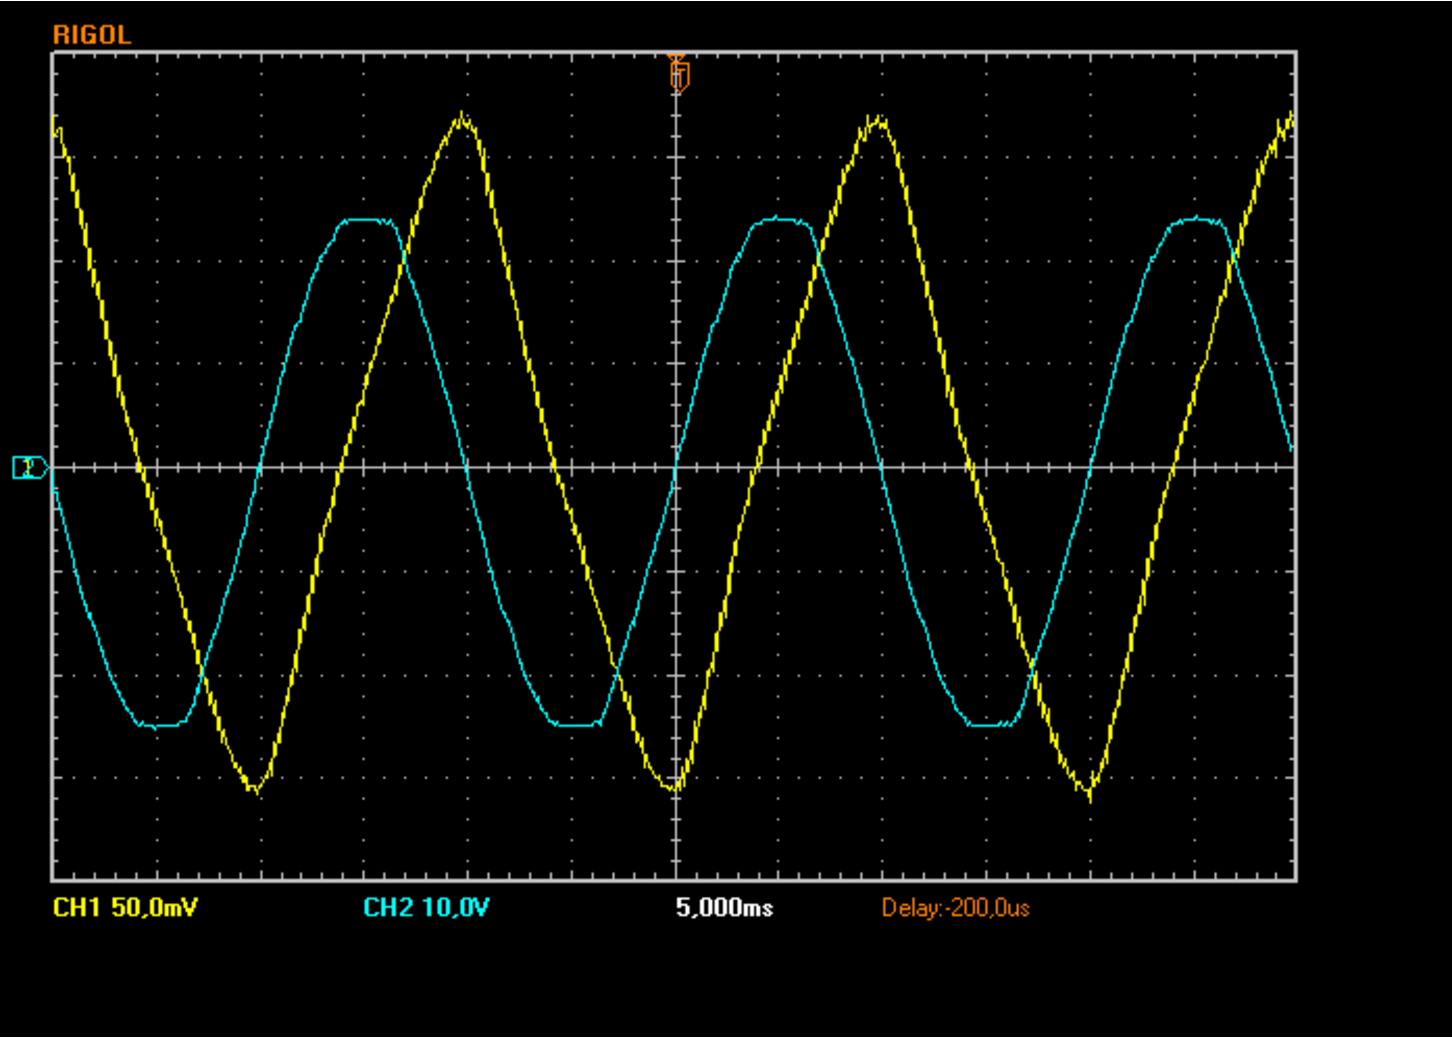
\includegraphics[width=0.95\textwidth]{./trafo/leerlauf.pdf}
	\end{center}
	\caption{Strom- Spannungverlauf bei Schaltung a, siehe \autoref{fig:abb9}.
		Die gelbe Kurve ist proportional zum Primärstrom und die blaue entspricht der Sekundärspannung}
	\label{fig:oszi_versuch1}
\end{figure}


\subsection{Ohm´sche Last}

Aus den aufgezeichneten Daten aus \autoref{tab:daten_versuch2} wurden nun die
geforderten Werte, wie in \autoref{tab:tab1} ersichtlich berechnet, die in folgender \autoref{tab:ergebnisse_versuch2}
aufgelistet sind.


\begin{table}[H]
	\caption{Gesuchte Größen, die anhand der gemessenen Werte aus
		\autoref{tab:daten_versuch2} berechnet wurden \\
		$S_1$ \dots Scheinleistung primär \\
		$Q_1$ \dots  Blindleistung\\
		$\lambda$ \dots Leistungsfaktor\\
		$P_2$ \dots Wirkleistung sekundär \\
		$P_V$ \dots Verlustleistung \\
		$\eta$ \dots Wirkungsgrad \\
		$\Delta$ \dots entsprechende Unsicherheit
	}
	\label{tab:ergebnisse_versuch2}
	\begin{center}
		\begin{tabular}{lrrrrrrrrrrrr}
	\toprule
	{} & $S_1$ / \si{\va}   & $\Delta S_1$ / \si{\va}   & $Q_1$ / \si{\var}  & $\Delta Q_1$ / \si{\var}  & $\lambda$ / 1          & $\Delta \lambda$ / 1          \\
	\midrule
	0  & 41.3               & 0.8                       & 32.7               & 1.1                       & 0.610                  & 0.015                         \\
	\bottomrule
	\toprule
	{} & $P_2$ / \si{\watt} & $\Delta P_2$ / \si{\watt} & $P_V$ / \si{\watt} & $\Delta P_V$ / \si{\watt} & $\eta$ / \si{\percent} & $\Delta \eta$ / \si{\percent} \\
	\midrule
	0  & 16.3               & 0.4                       & 8.9                & 0.5                       & 64.5                   & 1.9                           \\
	\bottomrule
\end{tabular}

	\end{center}
\end{table}

Außerdem wurden wieder die Sekundärspannung, sowie der Primärstrom mithilfe des
Oszilloskops aufgezeichnet und mithilfe des Analyseprogramms ``Ultrascope``
folgende \autoref{fig:oszi_versuch2} erzeugt.

\begin{figure}[H]
	\begin{center}
		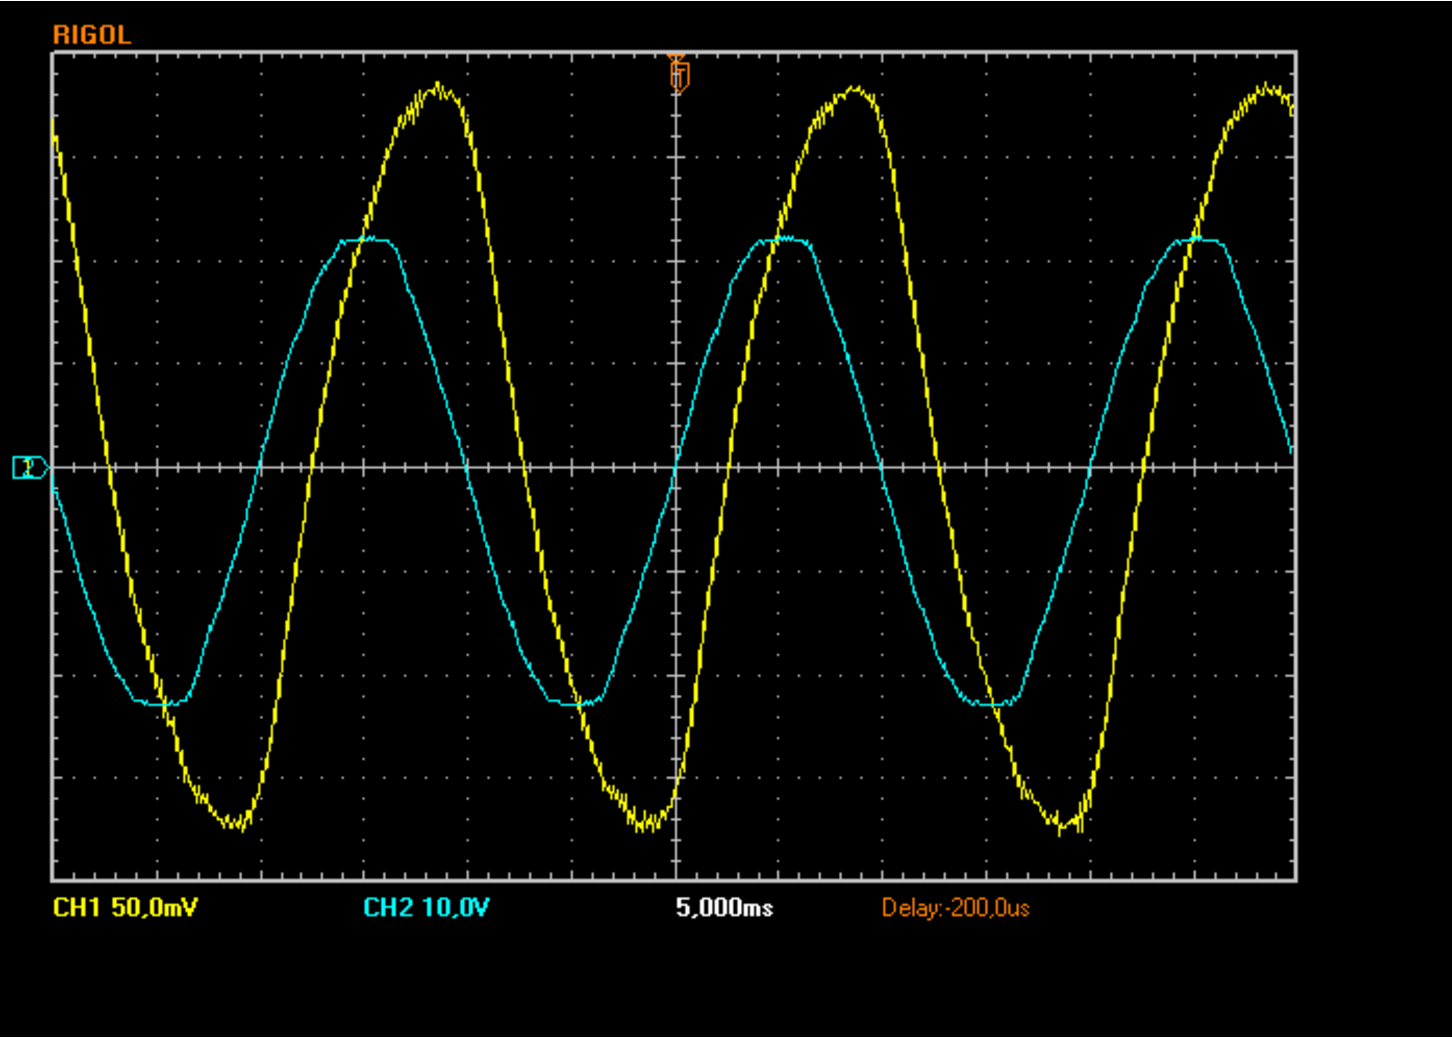
\includegraphics[width=0.95\textwidth]{./trafo/widerstand.pdf}
	\end{center}
	\caption{Strom- Spannungverlauf bei Schaltung b, siehe \autoref{fig:abb9}.
		Die gelbe Kurve ist proportional zum Primärstrom und die blaue entspricht der Sekundärspannung}
	\label{fig:oszi_versuch2}
\end{figure}



\subsection{Ohm´sch-induktive Last}

Damit die Wirkleistungsabgabe am Widerstand maximiert wird, wird folgende \autoref{eq:widerstandleistung}
\begin{equation}
	P_R = U_R I_2 =  \frac{U_2^2}{R_L^2 + X_L^2} R_L
	\label{eq:widerstandleistung}
\end{equation}
nach dem Widerstand abgeleitet und null gesetzt so kommt man darauf, dass bei
\begin{equation}
	R_L = X_L
	\label{eq:}
\end{equation}
die Wirkleistungsabgabe am Widerstand maximal ist. Weiters wurde der
Lastwiderstand indirekt gemessen, indem der Spannungsabfall über den
Widerstand $U_R$ und der Sekundärstrom $I_2$ gemessen wurde, somit ist:
\begin{equation}
	R_L = \frac{U_R}{I_2}
	\label{eq:lastwiderstandglg}
\end{equation}
Diese \autoref{eq:widerstandleistung} kann nun auch mit den gemessenen Daten
der Wirkleistung am Widerstand zum Widerstand gefittet werden.

Zunächst werden aus den aufgezeichneten Daten aus \autoref{tab:daten_versuch3} der
Lastwiderstand $R_L$ und die Wirkleistung am Widerstand $P_R$ berechnet. Wodurch die in folgender
\autoref{tab:ergebnisse_versuch3} aufgelisteten Ergebnissen entstehen.


\begin{table}[H]
	\caption{Erhaltenen Werte für den Lastwiderstand
		und die Wirkleistung am Lastwiderstand unter Verwendung der Daten aus
		\autoref{tab:daten_versuch3}, anhand \autoref{eq:lastwiderstandglg}
		und \autoref{eq:widerstandleistung}  \\
		$R_L$ \dots Lastwiderstand \\
		$P_R$ \dots Wirkleistung am Lastwiderstand \\
		$\Delta$ \dots entsprechende Unsicherheit
	}
	\label{tab:ergebnisse_versuch3}
	\begin{center}
		\begin{tabular}{lrrrr}
	\toprule
	{} & $P_R$ / \si{\watt} & $\Delta P_R$ / \si{\watt} & $R_L$ / \si{\ohm} & $\Delta R_L$ / \si{\ohm} \\
	\midrule
	0  & 0.61               & 0.05                      & 1.81              & 0.13                     \\
	1  & 1.34               & 0.06                      & 4.29              & 0.19                     \\
	2  & 1.62               & 0.07                      & 5.2               & 0.2                      \\
	3  & 2.17               & 0.08                      & 7.2               & 0.3                      \\
	4  & 2.65               & 0.09                      & 9.1               & 0.3                      \\
	5  & 2.99               & 0.10                      & 10.9              & 0.4                      \\
	6  & 3.37               & 0.13                      & 12.9              & 0.5                      \\
	7  & 3.67               & 0.14                      & 15.3              & 0.6                      \\
	8  & 3.74               & 0.14                      & 16.3              & 0.7                      \\
	9  & 4.00               & 0.15                      & 18.9              & 0.7                      \\
	10 & 4.16               & 0.16                      & 21.0              & 0.8                      \\
	11 & 4.30               & 0.16                      & 23.3              & 0.9                      \\
	12 & 4.31               & 0.17                      & 25.6              & 1.0                      \\
	13 & 4.34               & 0.17                      & 27.1              & 1.1                      \\
	14 & 4.49               & 0.17                      & 29.5              & 1.2                      \\
	15 & 4.37               & 0.17                      & 30.3              & 1.2                      \\
	16 & 4.28               & 0.18                      & 33.1              & 1.4                      \\
	17 & 4.3                & 0.3                       & 37.1              & 1.9                      \\
	18 & 4.3                & 0.3                       & 37.4              & 1.9                      \\
	19 & 4.2                & 0.3                       & 40                & 3                        \\
	20 & 4.2                & 0.3                       & 41                & 3                        \\
	21 & 4.2                & 0.3                       & 43                & 3                        \\
	22 & 4.1                & 0.3                       & 45                & 3                        \\
	\bottomrule
\end{tabular}

	\end{center}
\end{table}


Diese Daten werden, wie zuvor erklärt, mit den Defaulteinstellungen des LMFIT
Python Moduls \cite{LmFitNewville2014} gefittet. Dies bedeutet, mit der Levenberg-Marquardt Methode als
Fitgüte, die Chi-Quadrat-Statistik ($\chi^2$) verwendet.
Normalerweise werden die 1$\sigma$ Unsicherheiten der Fit-Parameter berechnet,
indem ein Fitparameter variiert wird, bis dieser eine Erhöhung von 1 in der
$\chi^2$ Statistik hervorruft. Jedoch ist dies nicht der Default von LMFIT.
LMFIT nimmt an, dass die Bestimmung der Unsicherheiten der Messungen nicht, oder
nur schwer möglich ist. Deshalb rechnet LMFIT die Unsicherheiten der Parameter
implizit, unter den Annahmen, dass der Fit ein guter ist und die Daten eine
normalverteilte Unsicherheit, um den eigentlichen Wert besitzen aus. Die implizite
Ausrechnung der Unsicherheiten eines Parameters geschieht, indem ein Parameter
variiert wird, bis diese Variation die $\chi^2$ um die reduzierte
Chi-Quadrat-Statistik erhöht. Die red. $\chi^2$ entspricht bei einem guten Fit
ungefähr 1 und somit der üblichen Methode der Berechnung der
Unsicherheit eines Fitparameters. Dies wird erreicht, indem bei der Optimierung
die Unsicherheiten der Daten, diese mit red. $\chi^2$ gewichtet werden. Dadurch ergibt
sich, dass die Unsicherheiten der Parameter eher dem wahren Wert der
Unsicherheit entsprechen, wenn der Fit ``gut`` ist. (Genaueres findet man
\href{https://lmfit.github.io/lmfit-py/fitting.html#uncertainties-in-variable-parameters-and-their-correlations}{hier}).
\vspace{2mm}
Somit erhält man folgende \autoref{fig:fit}.

\begin{figure}[H]
	\begin{center}
		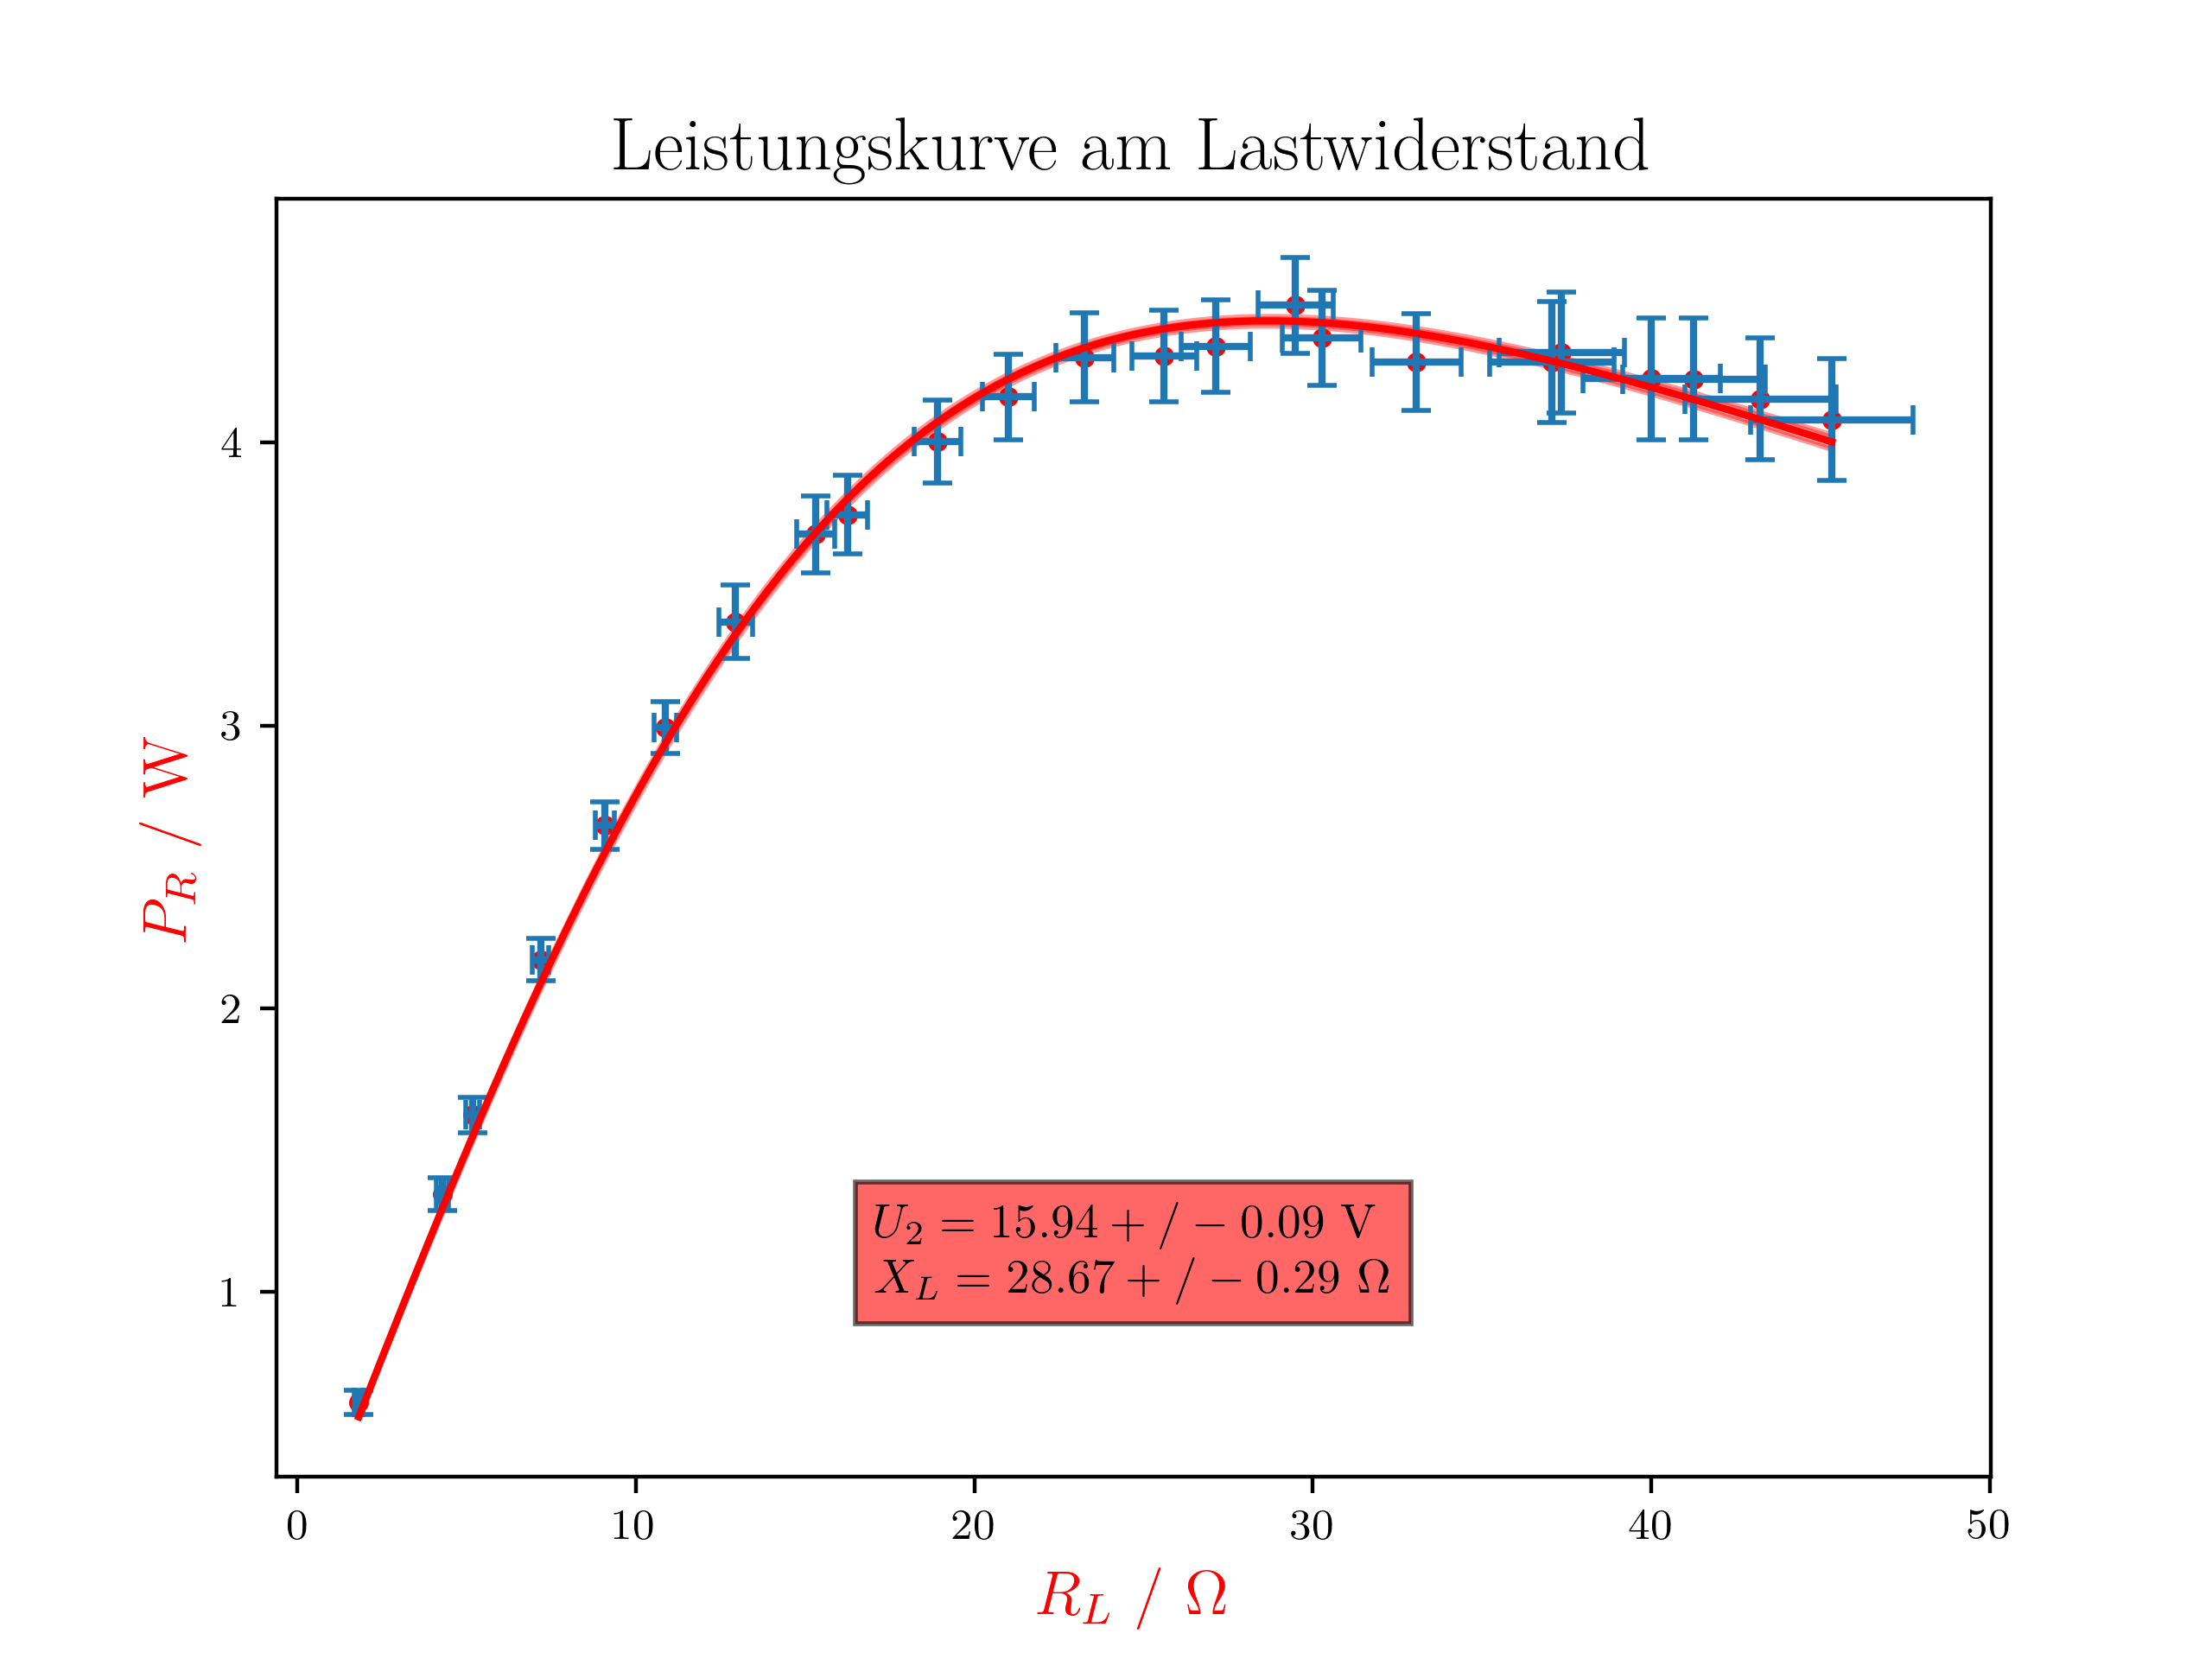
\includegraphics[width=0.95\textwidth]{./bigpics/original.png}
	\end{center}
	\caption{Fit der gemessenen Daten aus \autoref{tab:ergebnisse_versuch3} mit
		\autoref{eq:widerstandleistung} wobei $R_L$ der Lastwiderstand und $P_L$ die
		Wirkleistung am Widerstand sind. $X_L$ ist der Fitparameter des
		Blindwiderstands und $U_2$ ist der Fitparameter der Klemmspannung der b Schaltung aus
		\autoref{fig:abb9}, mit Defaulteinstellungen des Python LMFIT Moduls}
	\label{fig:fit}
\end{figure}

Jedoch ist es auch möglich eigene Wichtungen durchzuführen. Hier wurden die
Daten mit $w=\frac{1}{\Delta P}$ gewichtet. Weiters kann die Skalierung der
Unsicherheit der Daten ausgeschaltet werden. Die Resultate dieser drei
zusätzlichen Einstellungen werden in folgenden Abbildungen dargestellt:

\begin{figure}[H]
	\begin{center}
		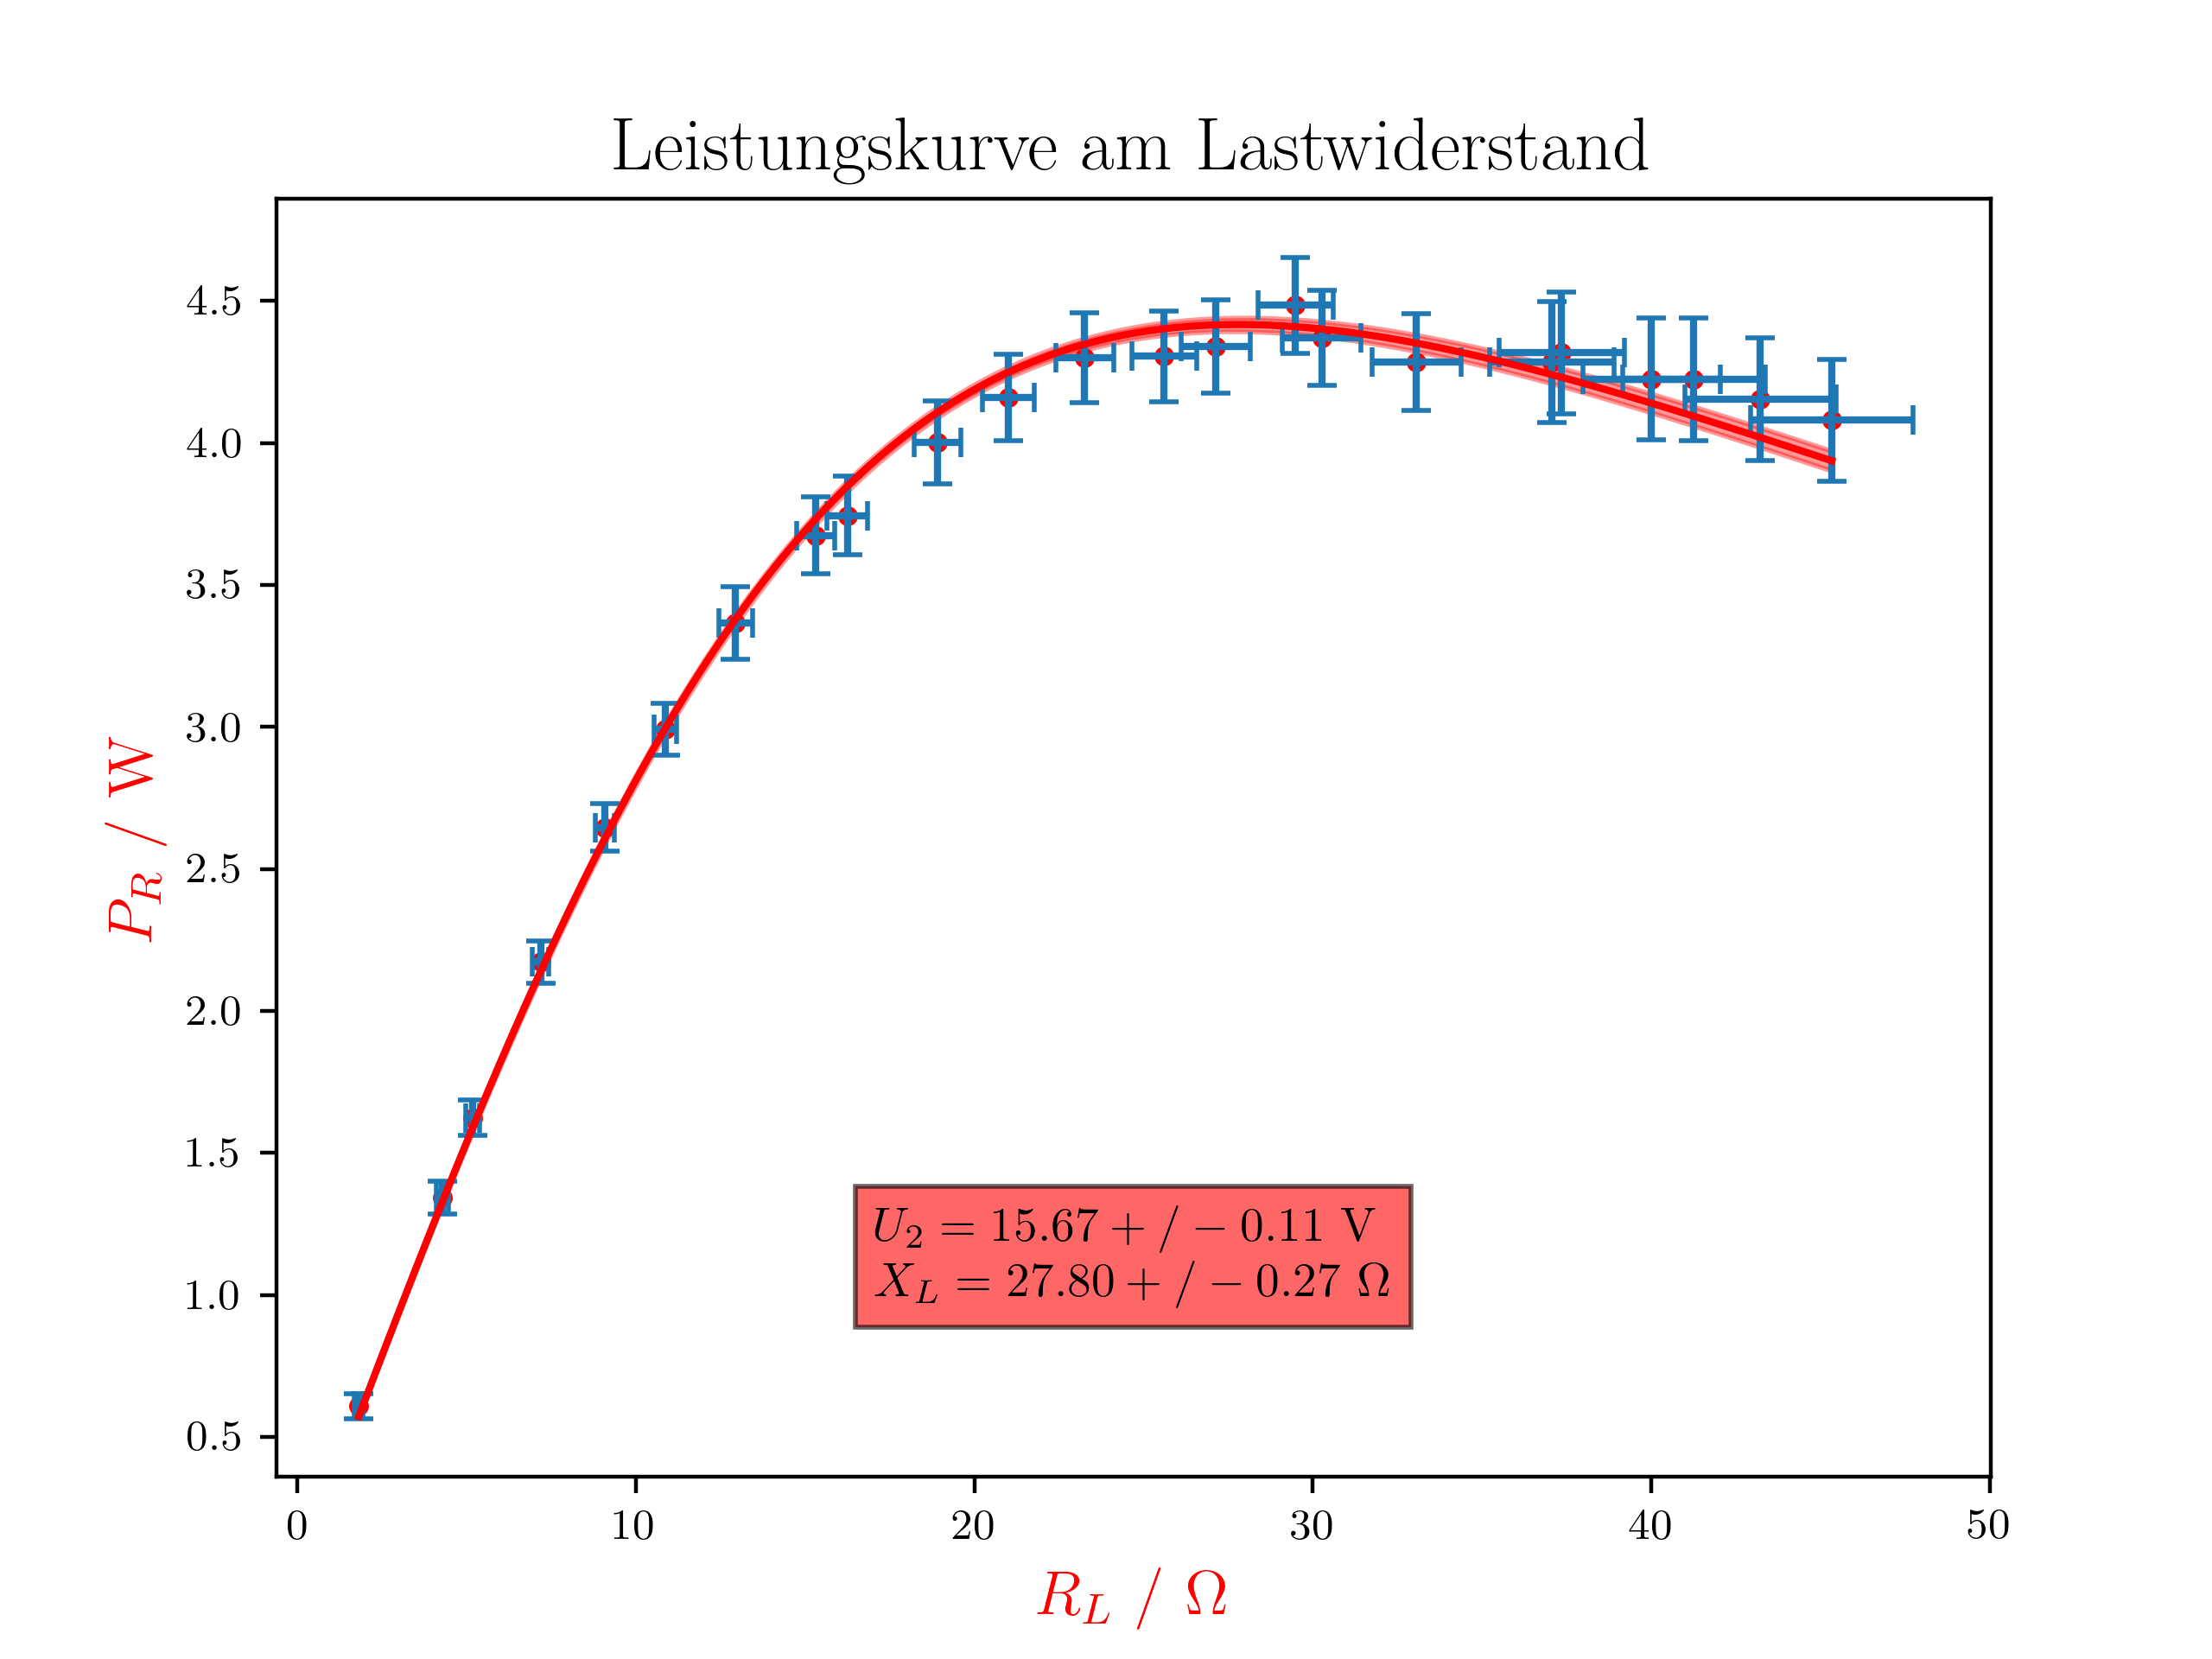
\includegraphics[width=0.95\textwidth]{./bigpics/withweightsandscalecovartrue.png}
	\end{center}
	\caption{Fit der gemessenen Daten aus \autoref{tab:ergebnisse_versuch3} mit
		\autoref{eq:widerstandleistung} wobei $R_L$ der Lastwiderstand und $P_L$ die
		Wirkleistung am Widerstand sind. $X_L$ ist der Fitparameter des
		Blindwiderstands und $U_2$ ist der Fitparameter der Klemmspannung der b Schaltung aus
		\autoref{fig:abb9}, mit Wichtung der Datenpunkte und mit Skalierung (\texttt{scale\_covar=True})}
	\label{fig:fit_mit_wichtung_mit_skalierung}
\end{figure}

\begin{figure}[H]
	\begin{center}
		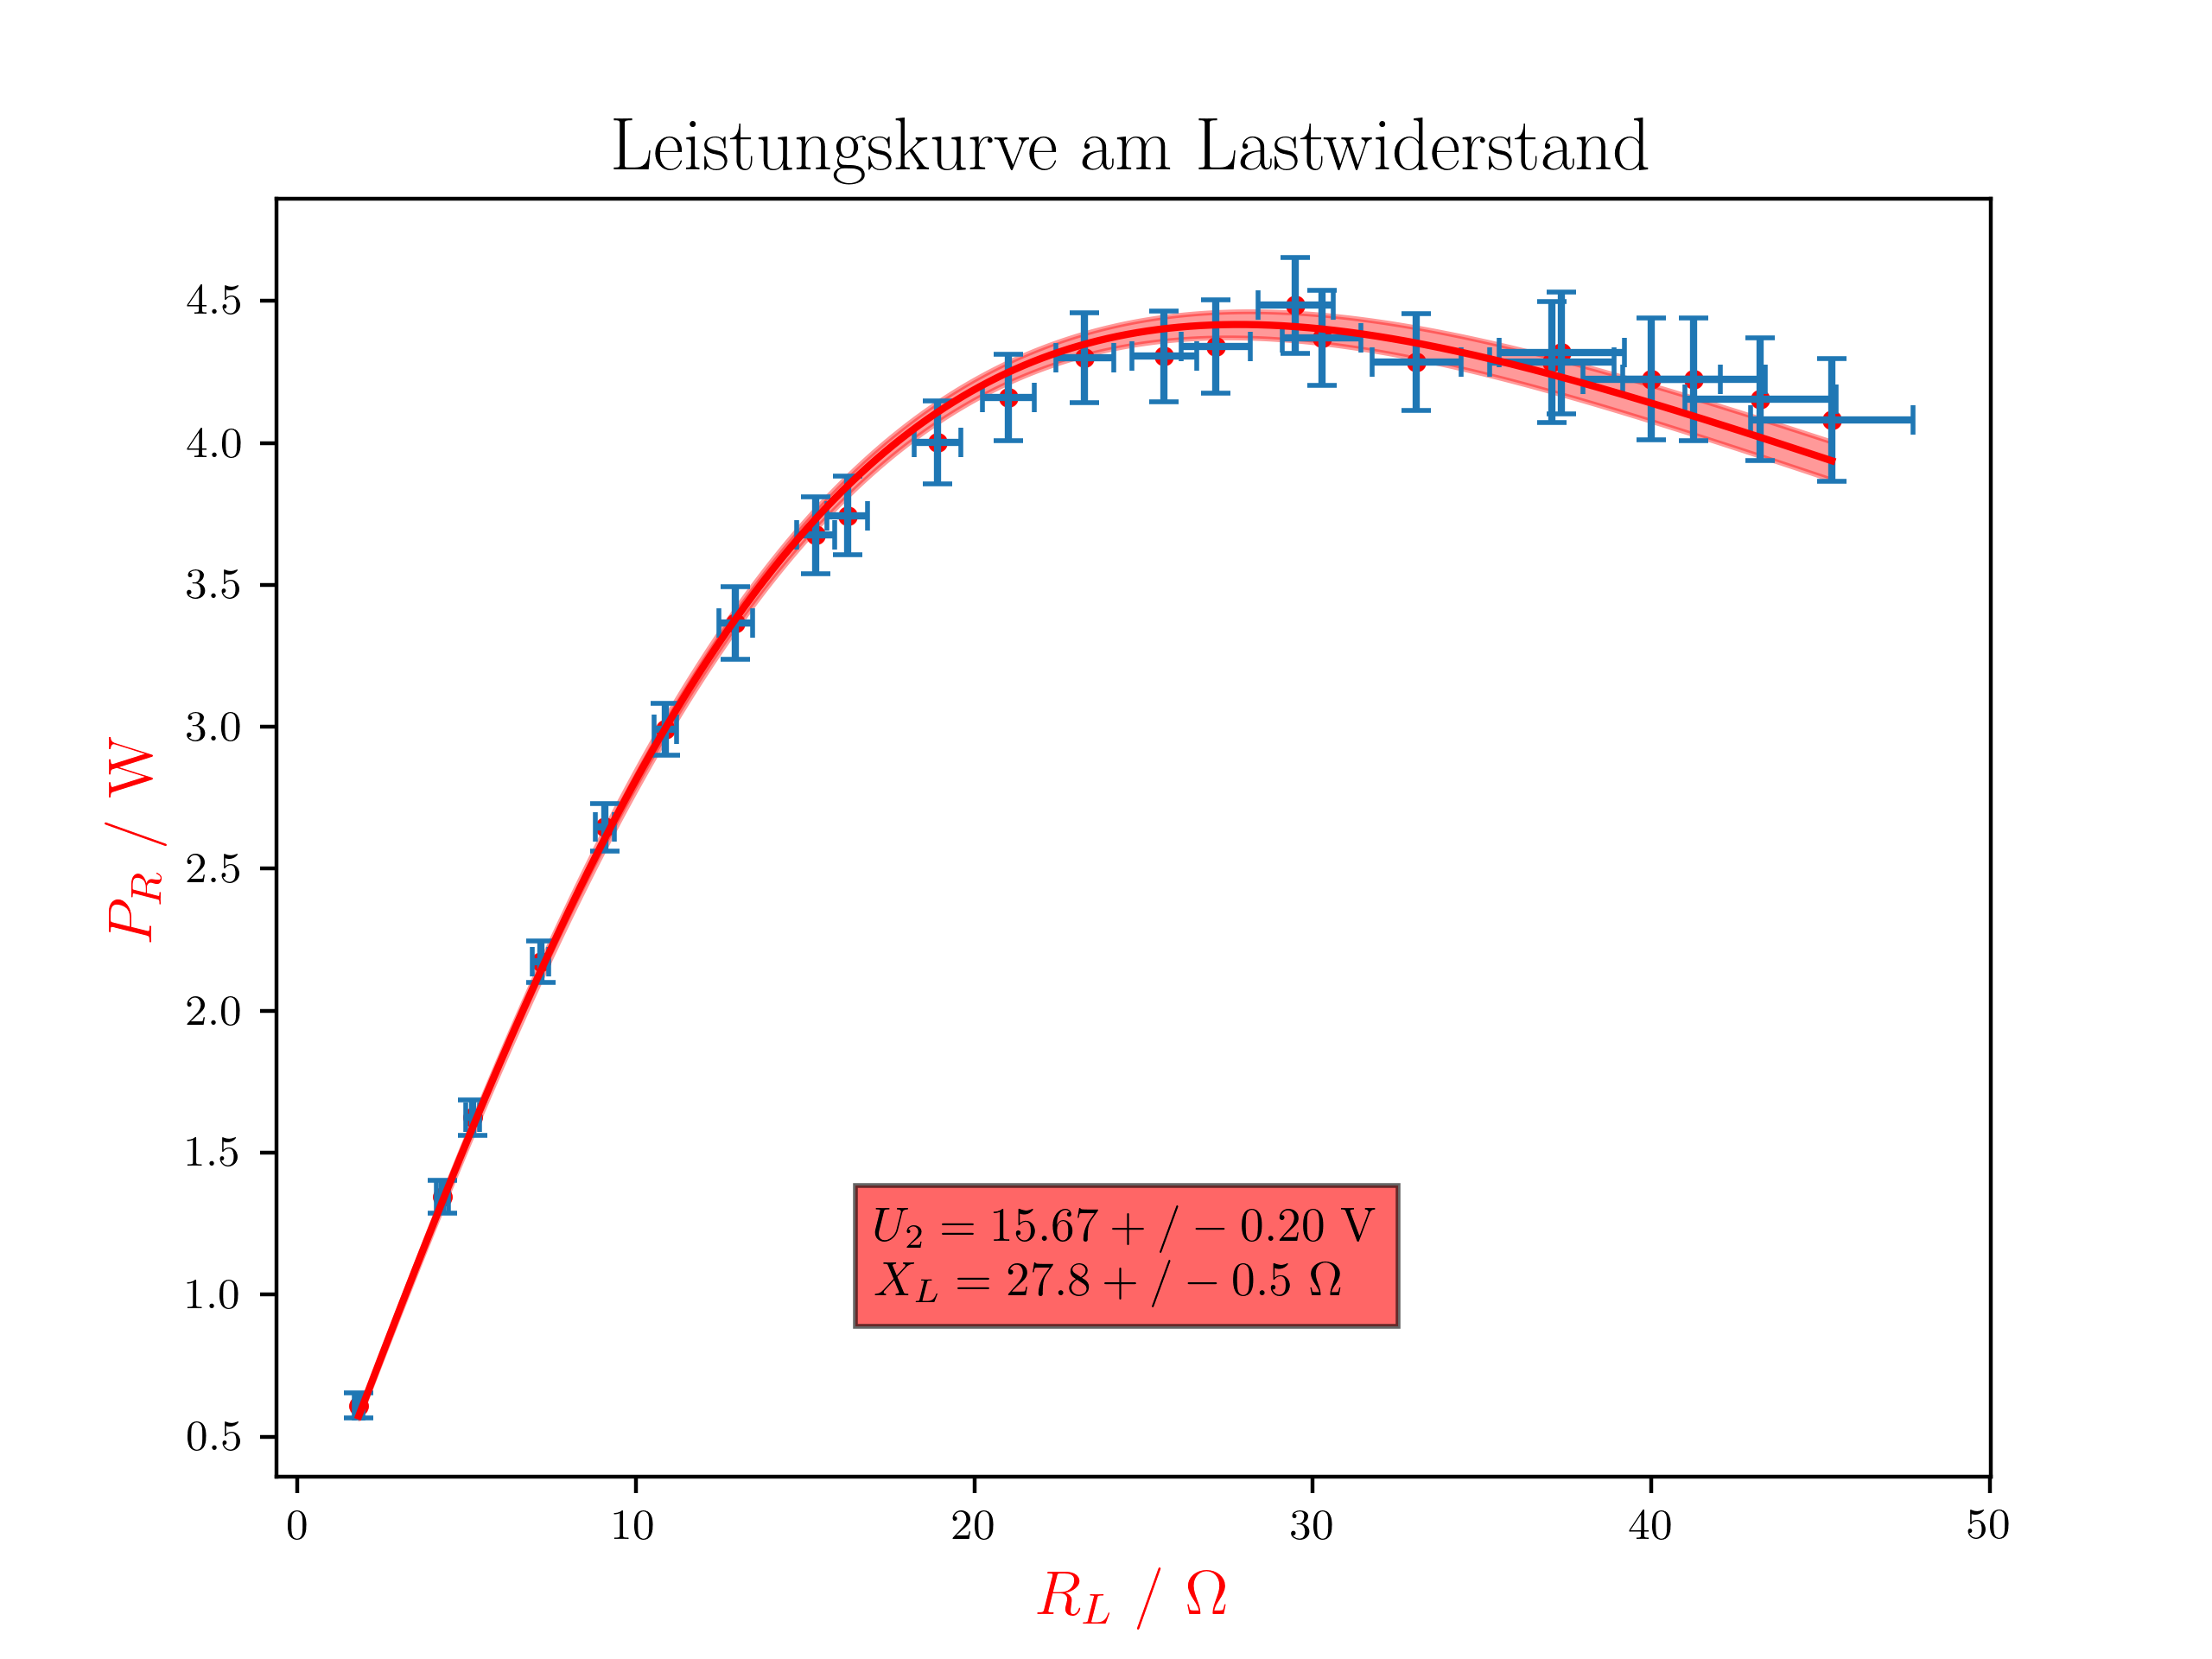
\includegraphics[width=0.95\textwidth]{./bigpics/withweightsandscalecovarfalse.png}
	\end{center}
	\caption{Fit der gemessenen Daten aus \autoref{tab:ergebnisse_versuch3} mit
		\autoref{eq:widerstandleistung} wobei $R_L$ der Lastwiderstand und $P_L$ die
		Wirkleistung am Widerstand sind. $X_L$ ist der Fitparameter des
		Blindwiderstands und $U_2$ ist der Fitparameter der Klemmspannung der b Schaltung aus
		\autoref{fig:abb9}, mit Wichtung der Datenpunkte und ohne Skalierung (\texttt{scale\_covar=False})}
	\label{fig:fit_mit_wichtung_ohne_skalierung}
\end{figure}

\begin{figure}[H]
	\begin{center}
		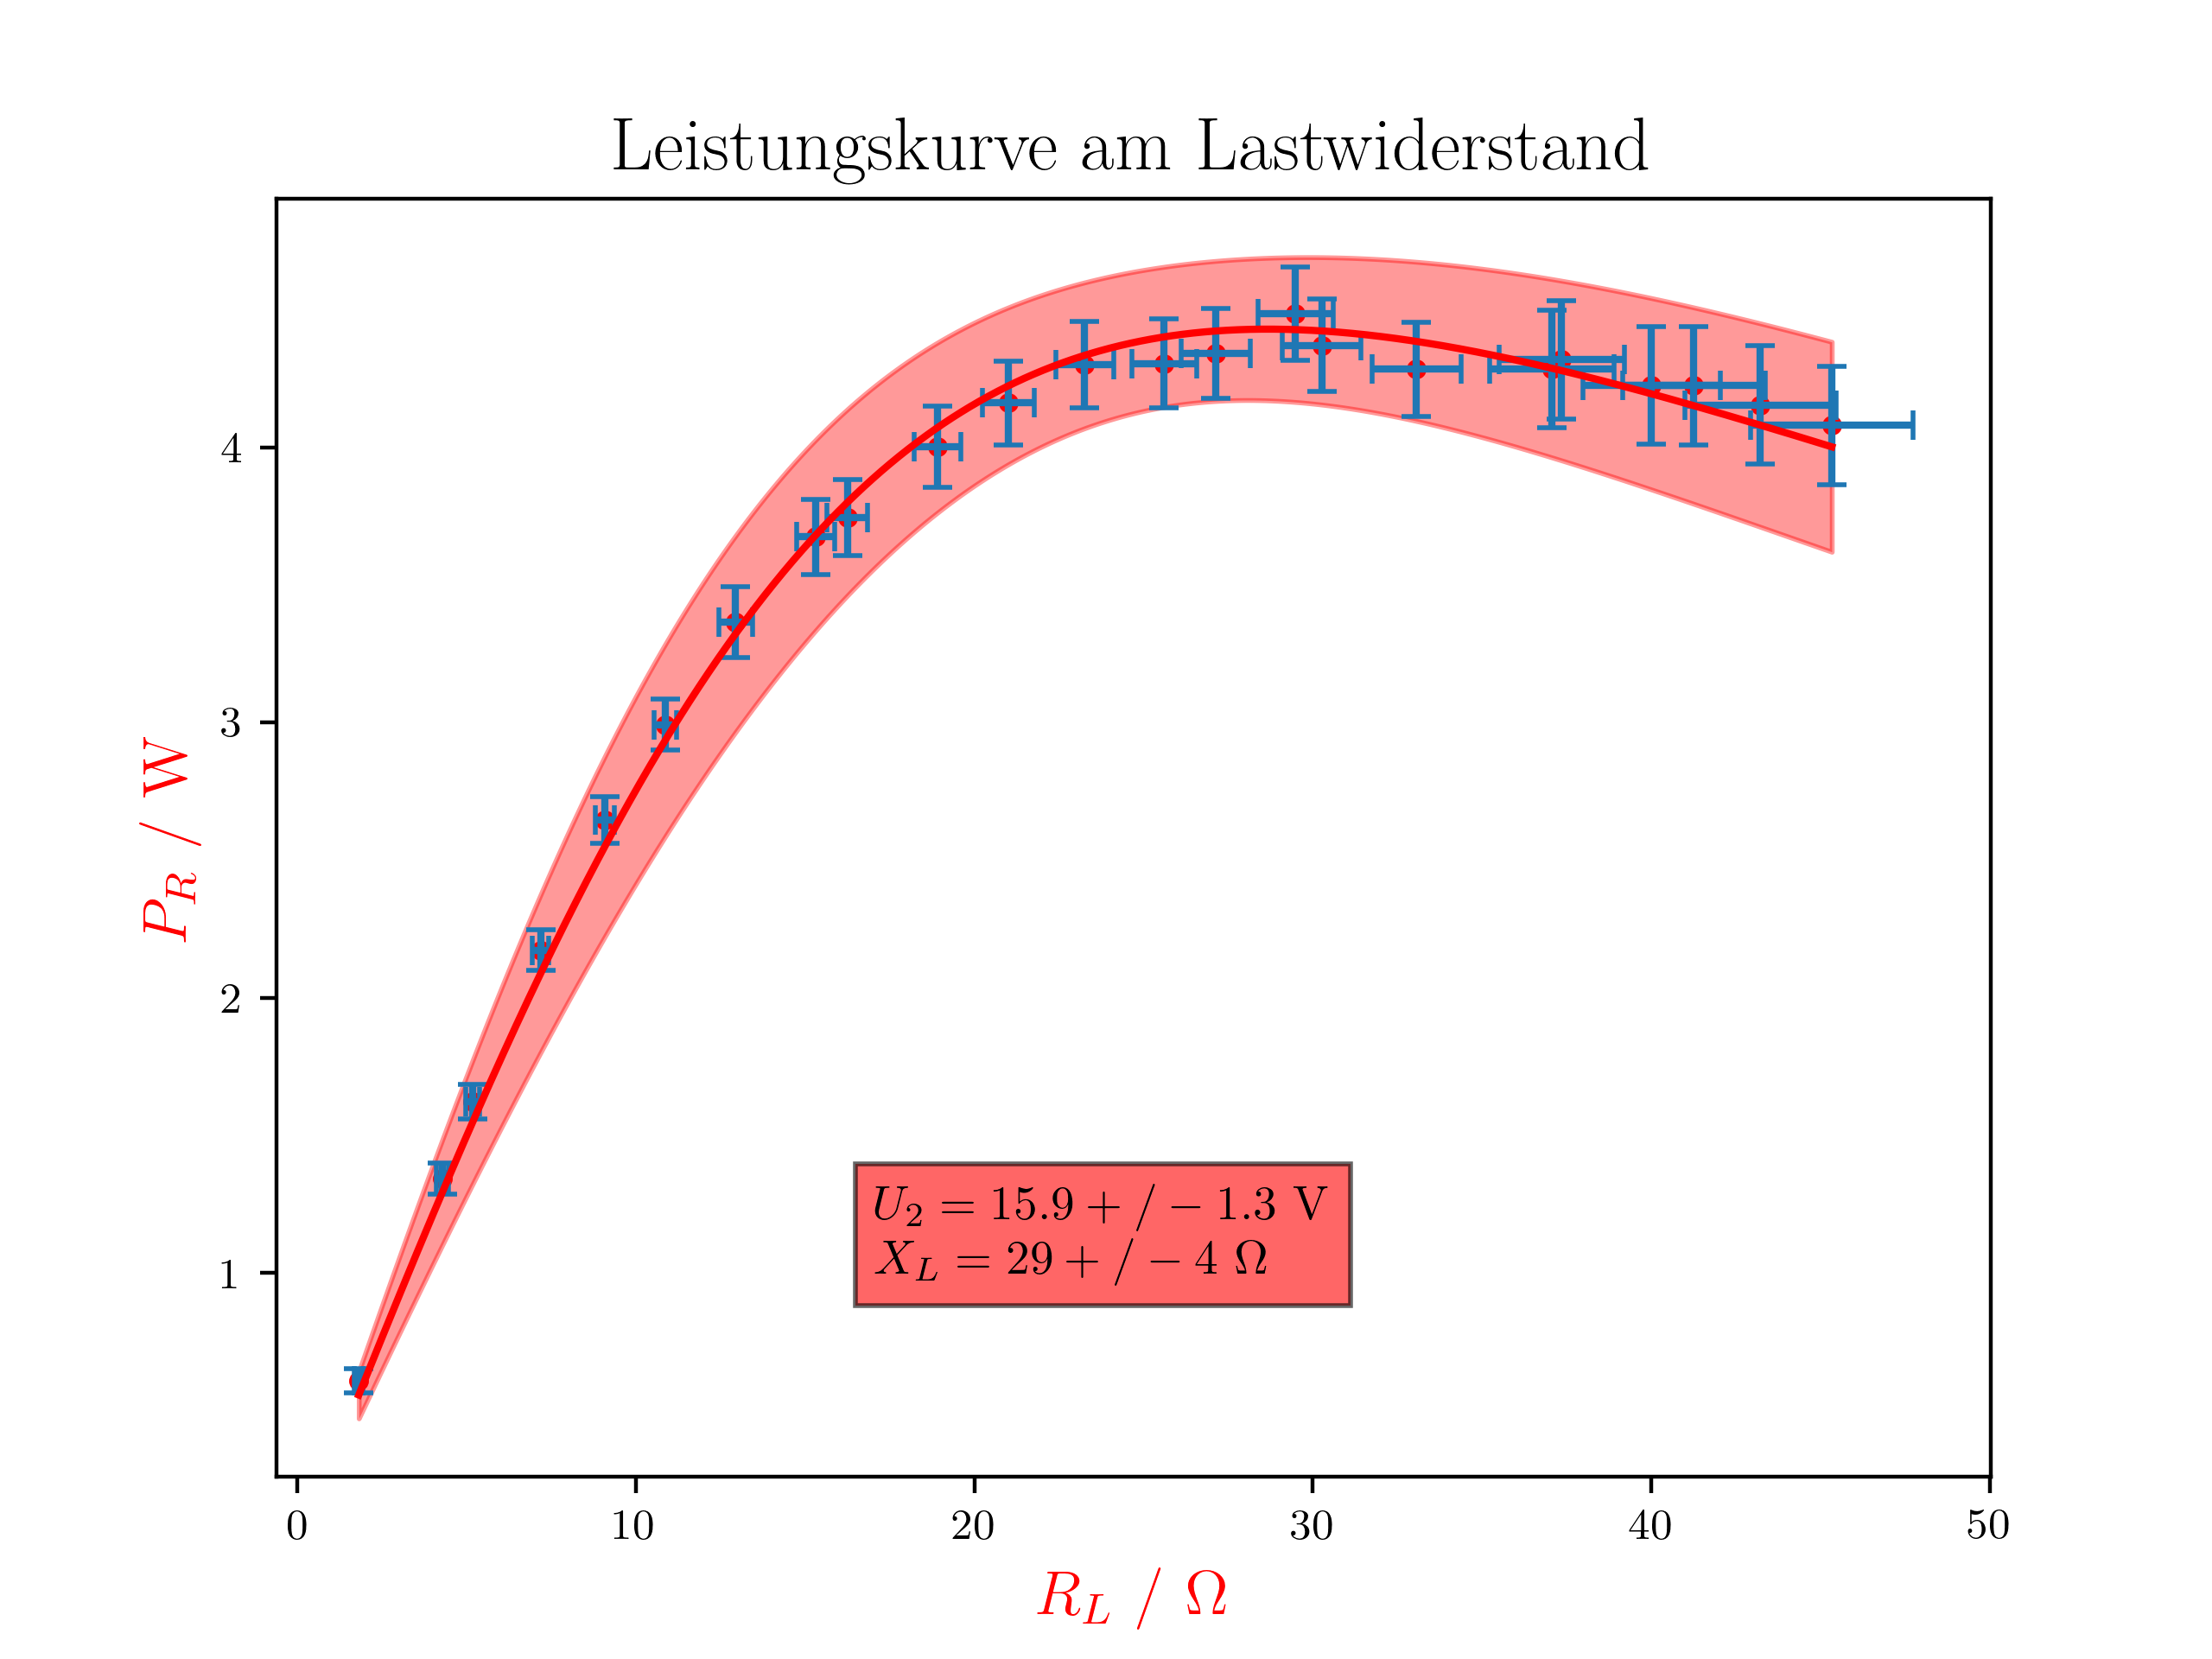
\includegraphics[width=0.95\textwidth]{./bigpics/withoutweigtsandscalecovarfalse.png}
	\end{center}
	\caption{Fit der gemessenen Daten aus \autoref{tab:ergebnisse_versuch3} mit
		\autoref{eq:widerstandleistung} wobei $R_L$ der Lastwiderstand und $P_L$ die
		Wirkleistung am Widerstand sind. $X_L$ ist der Fitparameter des
		Blindwiderstands und $U_2$ ist der Fitparameter der Klemmspannung der b Schaltung aus
		\autoref{fig:abb9}, mit ohne Wichtung der Datenpunkte und ohne Skalierung (\texttt{scale\_covar=False})}
	\label{fig:fit_ohne_wichtung_ohne_skalierung}
\end{figure}
%*unsicherheiten

%*

\vspace{2mm}

Zusätzlich werden noch die Werte aus \autoref{tab:tab1} mittels den Daten aus
\autoref{tab:daten_versuch3} berechnet. Um jedoch den Wirkungsgrad von der Leistung am Widerstand zu bestimmen wurde
dieser anders berechnet, wie unten beschrieben, gleiches gilt für die
Verlustleistung, alles was nicht am Widerstand abgegeben wird, ist Verlust.

\begin{table}[H]
	\caption{Gesuchte Größen, die anhand der gemessenen Werte aus
		\autoref{tab:daten_versuch3} berechnet wurden \\
		$S_1$ \dots Scheinleistung primär \\
		$Q_1$ \dots  Blindleistung \\
		$\lambda$ \dots Leistungsfaktor \\
		$\Delta$ \dots entsprechende Unsicherheit
	}
	\label{tab:ergebnisse_versuch3_extra}
	\begin{center}
		\begin{tabular}{lrrrrrrrrrrrr}
	\toprule
	{} & $S_1$ / \si{\va} & $\Delta S_1$ / \si{\va} & $Q_1$ / \si{\var} & $\Delta Q_1$ / \si{\var} & $\lambda$ / 1 & $\Delta \lambda$ / 1 \\
	\midrule
	0  & 43.2             & 0.8                     & 42.1              & 0.9                      & 0.222         & 0.007                \\
	1  & 43.2             & 0.8                     & 41.9              & 0.9                      & 0.238         & 0.007                \\
	2  & 43.2             & 0.8                     & 41.9              & 0.9                      & 0.245         & 0.007                \\
	3  & 42.8             & 0.8                     & 41.3              & 0.9                      & 0.259         & 0.008                \\
	4  & 42.4             & 0.8                     & 40.8              & 0.9                      & 0.271         & 0.008                \\
	5  & 42.4             & 0.8                     & 40.7              & 0.9                      & 0.276         & 0.008                \\
	6  & 42.4             & 0.8                     & 40.6              & 0.9                      & 0.285         & 0.008                \\
	7  & 41.6             & 0.8                     & 39.7              & 0.9                      & 0.298         & 0.008                \\
	8  & 41.3             & 0.8                     & 39.4              & 0.9                      & 0.298         & 0.008                \\
	9  & 40.5             & 0.8                     & 38.5              & 0.9                      & 0.309         & 0.009                \\
	10 & 40.5             & 0.8                     & 38.5              & 0.9                      & 0.309         & 0.009                \\
	11 & 39.7             & 0.8                     & 37.7              & 0.9                      & 0.315         & 0.009                \\
	12 & 39.3             & 0.8                     & 37.2              & 0.9                      & 0.318         & 0.009                \\
	13 & 38.9             & 0.8                     & 36.8              & 0.8                      & 0.322         & 0.009                \\
	14 & 38.9             & 0.8                     & 36.8              & 0.8                      & 0.322         & 0.009                \\
	15 & 38.9             & 0.8                     & 36.8              & 0.8                      & 0.319         & 0.009                \\
	16 & 38.1             & 0.8                     & 36.0              & 0.8                      & 0.326         & 0.009                \\
	17 & 37.7             & 0.8                     & 35.6              & 0.8                      & 0.324         & 0.009                \\
	18 & 37.7             & 0.8                     & 35.6              & 0.8                      & 0.324         & 0.009                \\
	19 & 37.3             & 0.8                     & 35.2              & 0.8                      & 0.325         & 0.009                \\
	20 & 37.3             & 0.8                     & 35.3              & 0.8                      & 0.322         & 0.009                \\
	21 & 37.3             & 0.8                     & 35.3              & 0.8                      & 0.319         & 0.009                \\
	22 & 36.5             & 0.7                     & 34.5              & 0.8                      & 0.324         & 0.009                \\
	\bottomrule
\end{tabular}

	\end{center}
\end{table}

\begin{table}[H]
	\caption{Gesuchte Größen, die anhand der gemessenen Werte aus
		\autoref{tab:daten_versuch3} berechnet wurden \\
		$R_L$ \dots Lastwiderstand\\
		$P_2$ \dots Wirkleistung sekundär \\
		$P_V = P_R - P_1$ \dots Verlustleistung \\
		$\eta = \frac{P_R}{P_1}$ \dots Wirkungsgrad \\
		$\Delta$ \dots entsprechende Unsicherheit
	}
	\label{tab:ergebnisse_versuch3_extra_cont}
	\begin{center}
		\begin{tabular}{lrrrrrrrrrrrr}
	\toprule
	{} & $R_L$ / \si{\ohm} & $\Delta R_L$ / \si{\ohm} & $P_2$ / \si{\watt} & $\Delta P_2$ / \si{\watt} & $P_V$ / \si{\watt} & $\Delta P_V$ / \si{\watt} & $\eta$ / \si{\percent} & $\Delta \eta$ / \si{\percent} \\
	\midrule
	0  & 1.81              & 0.13                     & 10.2               & 0.4                       & 8.99               & 0.15                      & 6.3                    & 0.6                           \\
	1  & 4.29              & 0.19                     & 9.7                & 0.4                       & 8.96               & 0.16                      & 13.0                   & 0.7                           \\
	2  & 5.2               & 0.2                      & 9.7                & 0.4                       & 8.98               & 0.17                      & 15.3                   & 0.8                           \\
	3  & 7.2               & 0.3                      & 9.6                & 0.4                       & 8.93               & 0.18                      & 19.6                   & 0.9                           \\
	4  & 9.1               & 0.3                      & 9.4                & 0.4                       & 8.85               & 0.19                      & 23.0                   & 1.0                           \\
	5  & 10.9              & 0.4                      & 9.1                & 0.4                       & 8.7                & 0.2                       & 25.6                   & 1.1                           \\
	6  & 12.9              & 0.5                      & 8.9                & 0.4                       & 8.7                & 0.3                       & 27.8                   & 1.3                           \\
	7  & 15.3              & 0.6                      & 8.4                & 0.3                       & 8.7                & 0.3                       & 29.6                   & 1.4                           \\
	8  & 16.3              & 0.7                      & 8.2                & 0.3                       & 8.6                & 0.3                       & 30.4                   & 1.4                           \\
	9  & 18.9              & 0.7                      & 7.9                & 0.3                       & 8.5                & 0.3                       & 32.0                   & 1.5                           \\
	10 & 21.0              & 0.8                      & 7.7                & 0.3                       & 8.3                & 0.3                       & 33.3                   & 1.5                           \\
	11 & 23.3              & 0.9                      & 7.4                & 0.3                       & 8.2                & 0.3                       & 34.4                   & 1.6                           \\
	12 & 25.6              & 1.0                      & 7.0                & 0.3                       & 8.2                & 0.3                       & 34.4                   & 1.6                           \\
	13 & 27.1              & 1.1                      & 6.8                & 0.3                       & 8.2                & 0.3                       & 34.7                   & 1.6                           \\
	14 & \color{red}29.5   & 1.2                      & 6.7                & 0.3                       & 8.0                & 0.3                       & \color{red}35.9        & 1.7                           \\
	15 & 30.3              & 1.2                      & 6.5                & 0.3                       & 8.0                & 0.3                       & 35.2                   & 1.7                           \\
	16 & 33.1              & 1.4                      & 6.2                & 0.3                       & 8.1                & 0.3                       & 34.5                   & 1.7                           \\
	17 & 37.1              & 1.9                      & 5.8                & 0.3                       & 7.9                & 0.4                       & 35                     & 3                             \\
	18 & 37.4              & 1.9                      & 5.8                & 0.3                       & 7.9                & 0.4                       & 35                     & 3                             \\
	19 & 40                & 3                        & 5.6                & 0.3                       & 7.9                & 0.4                       & 35                     & 3                             \\
	20 & 41                & 3                        & 5.5                & 0.3                       & 7.8                & 0.4                       & 35                     & 3                             \\
	21 & 43                & 3                        & 5.3                & 0.3                       & 7.7                & 0.4                       & 35                     & 3                             \\
	22 & 45                & 3                        & 5.1                & 0.3                       & 7.7                & 0.4                       & 35                     & 3                             \\
	\bottomrule
\end{tabular}

	\end{center}
\end{table}

Der Wert mit dem besten Wirkungsgrad ist derselbe Wert bei dem die Wirkleistung
am Widerstand am höchsten in der Tabelle ist, dieser Widerstandswert ist
\begin{align*}
	R_L = \SI{29.5(12)}{\ohm}
\end{align*}

Nun wird auch am Oszilloskop die Sekundärspannung sowie der Primärstrom des so
bestimmten Widerstands für das Maximum der Wirkleistung aufgezeichnet, wodurch
folgender Graph mithilfe des Programms ``Ultrascope`` erzeugt wird.


\begin{figure}[H]
	\begin{center}
		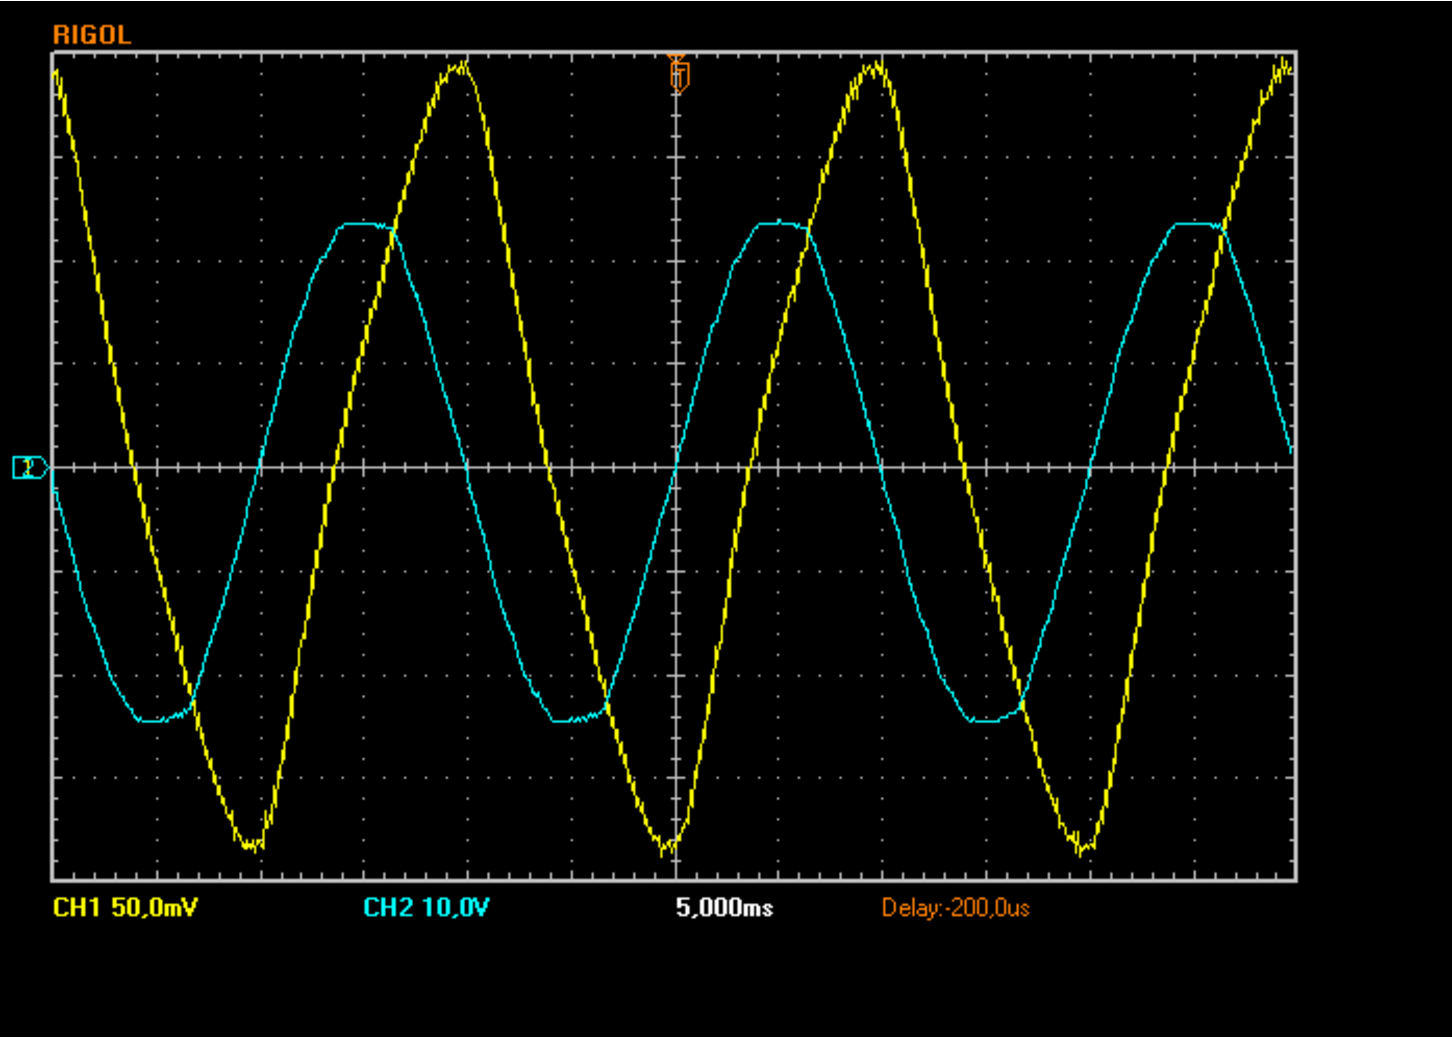
\includegraphics[width=0.95\textwidth]{./trafo/maxleistung.pdf}
	\end{center}
	\caption{Strom- Spannungverlauf bei Schaltung c, siehe \autoref{fig:abb9}.
		Die gelbe Kurve ist proportional zum Primärstrom und die blaue entspricht der Sekundärspannung}
	\label{fig:oszi_versuch3}
\end{figure}



\section{Diskussion}\label{disk}


\subsection{Leerlauf}

Anhand der Werte aus \autoref{tab:ergebnisse_versuch1} wird ersichtlich,
dass ein Großteil der Scheinleistung in der Bildleistung steckt. Dieses
Ergebnis spiegelt sich an der aufgezeichneten Grafik des Oszilloskops wieder,
da die Spannung und der Strom um \SI{90}{\degree} phasenverschoben sind, was
daran ersichtlich ist, dass beim Maximum der Einen Kurve, ein Nulldurchgang bei
der Anderen verzeichnet wird. Zusätzlich ist noch ersichtlich, dass der Merkspruch
``Induktor Spannung geht vor!´´ für das Vorzeichen der Phasenverschiebung
stimmt.


\subsection{Ohm´sche Last}

Aufgrund der zusätzlichen Ohm'schen Last ändert sich die Phasenbeziehung
zwischen Strom und Spannung. Weiters fließt ein stärkerer Strom, was wiederum
eine größere Scheinleistung verursacht. Ferner wird auch ersichtlich, dass sich
die Scheinleistung nicht nur aus der Bildleistung zusammensetzt. Diese Aussagen
werden auch durch den Anstieg des Betrags des Leistungsfaktors $\lambda$ von
\num{0.23(3)} aus \autoref{tab:ergebnisse_versuch1} zu \num{0.610(15)} aus
\autoref{tab:ergebnisse_versuch2} verifiziert.


\subsection{Ohm´sch-induktive Last}

Ein Maximum ist vorhanden, weil \autoref{eq:widerstandleistung}, wenn sie
abgeleitet wird, eine Nullstelle besitzt, und an dieser eine negative Krümmung
aufweist, wie auch anhand der Daten, aus \autoref{tab:daten_versuch3} und
\autoref{tab:daten_versuch3_2}, ersichtlich ist.

Durch die Wichtung der gemessenen Werte wird der Fit linkslastiger, da die
rechten Werte höhere Unsicherheiten besitzen. Dies ist in
\autoref{fig:fit_mit_wichtung_mit_skalierung} und
\autoref{fig:fit_mit_wichtung_ohne_skalierung} klar ersichtlich.

Es wurden vier verschiedene Einstellungen für das Fitten untersucht,
welche nun die plausibelste ist, hängt davon ab, wie korrekt die ermittelten
Unsicherheiten der Datenpunkte sind.

Der erste Fit, siehe \autoref{fig:fit}, mit den Defaulteinstellungen, sollte nur verwendet werden, wenn
keine Information zu den Unsicherheiten der Daten gegeben ist.

Der zweite Fit, siehe \autoref{fig:fit_mit_wichtung_mit_skalierung}, sollte
verwendet werden, wenn Information über die Unsicherheit der Daten vorhanden
ist, die Exaktheit dieser aber bezweifelt wird.

Der dritte Fit, siehe \autoref{fig:fit_mit_wichtung_ohne_skalierung}, sollte
verwendet werden, wenn Information über die Unsicherheit der Daten vorhanden
ist und sowohl Exaktheit, als auch Korrektheit dieser gegeben sind.

Der vierte Fit, siehe \autoref{fig:fit_ohne_wichtung_ohne_skalierung}, sollte
laut Dokumentation von LMFIT \cite{LmFitNewville2014} nicht verwendet werden.

Für diesen Versuch entspricht der dritten Fit am Besten den Gegebenheiten,
obwohl \autoref{fig:fit} einen besseren Fit liefert.

Da der dritte Fit den Gegebenheiten am besten entspricht, wird aus dieser
Fitkurve, siehe \autoref{fig:fit_mit_wichtung_ohne_skalierung}, der
Fitparameter $X_L$ entnommen. Dessen Wert entspricht auch dem, wie vorher
erläutert, Lastwiderstand, welcher die Wirkleistung maximiert. Der erhaltene Wert liegt
bei \SI{27.8(5)}{\ohm}.

Da der Wert für die Induktivität der Spule mit ungefähr $L \approx
	\SI{0.1}{\henry}$ und keine Unsicherheit angeben ist, wird die Unsicherheit
mit \SI{10}{\percent} abgeschätzt ($L = \SI{0.10(1)}{\henry}$). Dadurch lässt
sich ein Vergleichswert, für den Widerstand mit der maximalen
Leistungsübertragung folgendermaßen bestimmen:
\begin{align*}
	R_{L_{Vgl}} = \omega L = \SI{31(4)}{\ohm}
\end{align*}
wobei die Kreisfrequenz $\omega = 2 \pi \SI{50}{\Hz}$ wäre.

Nun wird noch eine Vergleichskurve mit den entsprechenden Unsicherheiten geplottet:
\begin{figure}[H]
	\begin{center}
		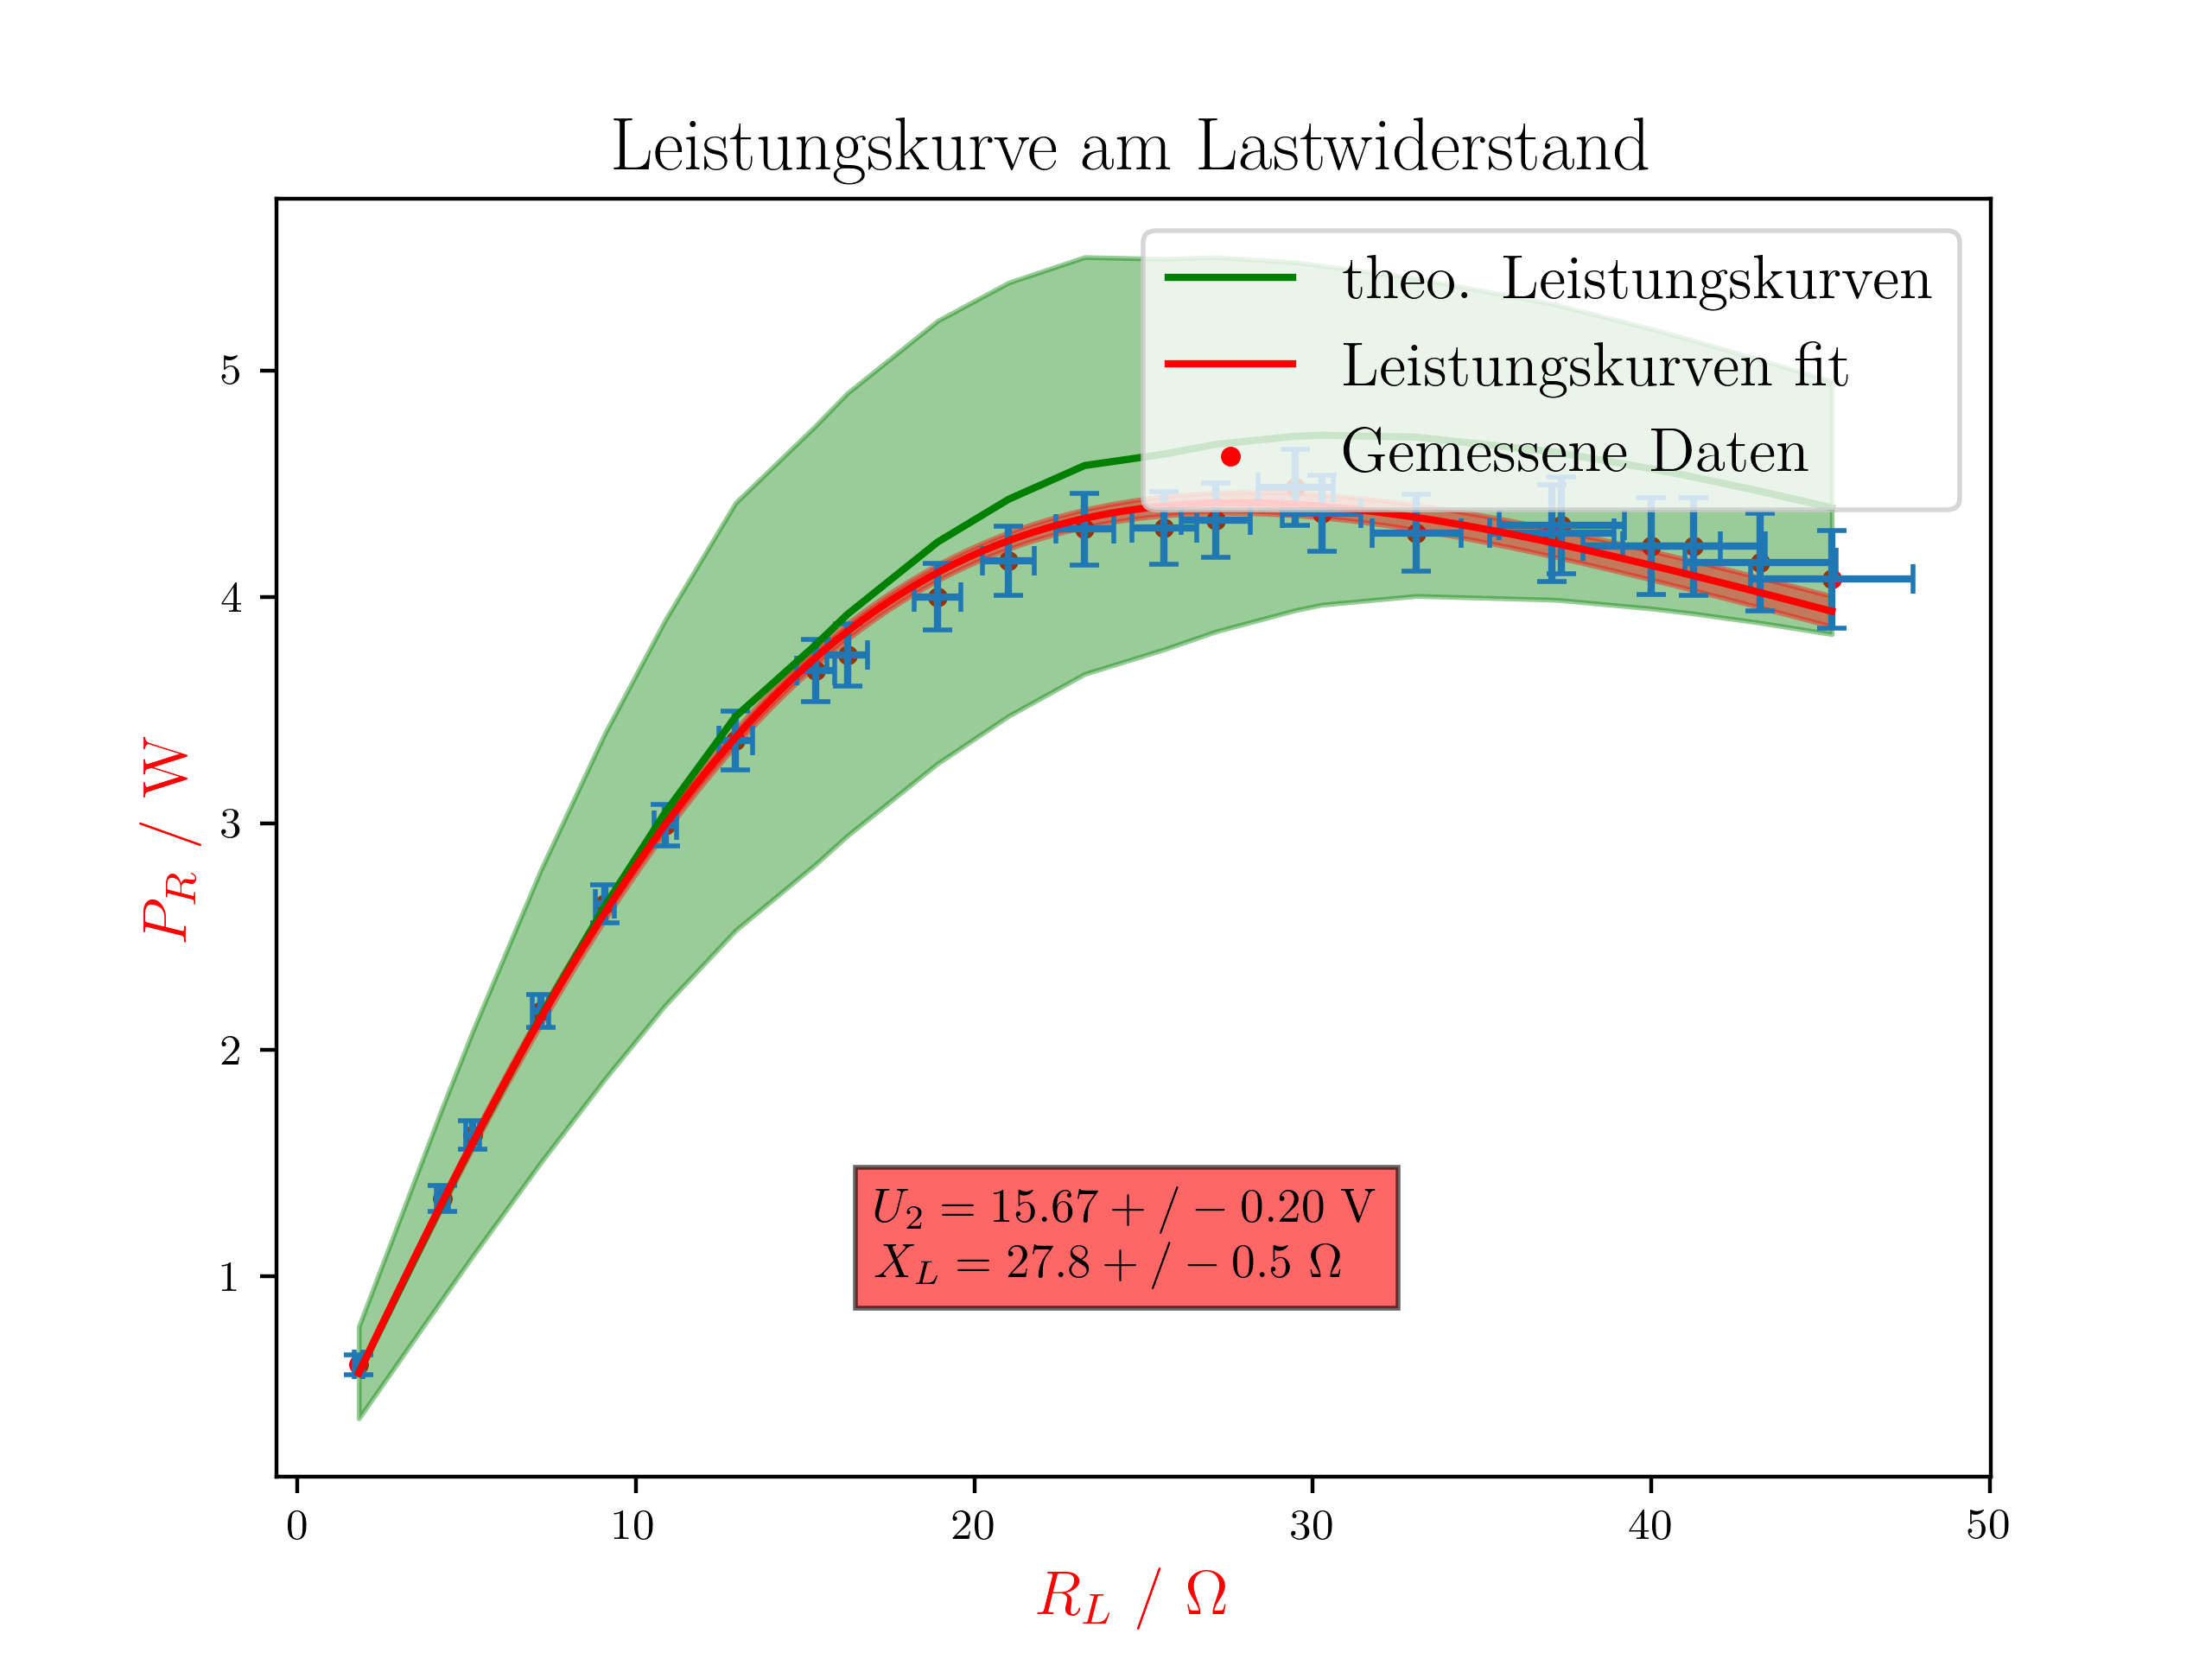
\includegraphics[width=0.95\textwidth]{./bigpics/vergleich}
	\end{center}
	\caption{Vergleich von der gefitteten Kurve (rot) mit der Vergleichskurve (grün)}
	\label{fig:vergleich}
\end{figure}

Wie in \autoref{fig:vergleich} ersichtlich, ist die gefittete Kurve im
Vergleichsintervall enthalten. Weiters is erkennbar, dass die linke Seite
besser mit dem Fit übereinstimmt als die Rechte.

\vspace{2mm}

Betrachtet man \autoref{fig:fit} ist klar ersichtlich, dass die Fitkurve in
allen Fehlerintervallen enthalten ist.

Anhand der Daten aus \autoref{tab:ergebnisse_versuch3_extra_cont} ist auch
ersichtlich, dass der Wirkungsgrad maximal wird, bei dem Wert, der durch den Fit
gegeben ist.


\subsection{Verbesserungsvorschläge}
Ein Verbesserungsvorschlag wäre die Verwendung von digitalen Multimetern um den
Ablesefehler zu umgehen.
Ein weiterer Vorteil wäre, dass die Kalibrierung der digitalen Messgeräte,
aufgrund von elektrischen Sicherheitsmechanismen, nicht bei Überlastungen, die
auf die Einstellung von zu kleinen Messbereichen zurückzuführen ist, verstellt wird.
Zudem kann die gesamte Datenaufzeichnung digital vonstatten gehen, damit in kurzer Zeit noch mehr
Wert zur Verfügung stehen würden, um den statistischen Fehler zu minimieren und auch menschliche Fehler auszuschließen.

\vspace{2mm}

Wenn die Induktivität der Spule bekannt wäre, könnte der theoretische Wert des
Widerstands, welcher die Wirkleistungsaufnahme maximiert, berechnet und
zum Vergleich herangezogen werden, wie bereits in 7.3 erwähnt. Zudem könnte eine theoretische Kurve für den
Leistungsverlauf erzeugt und mit der gemessenen Fitkurve grafisch verglichen
werden.





\section{Zusammenfassung}

Die erhaltenen Ergebnisse sind im folgenden nochmals aufgelistet.

\begin{table}[H]
	\caption{Zusammenfassende Tabelle aller erhaltenen Werte \\
		$S_1$ \dots Scheinleistung primär \\
		$Q_1$ \dots  Blindleistung\\
		$\lambda$ \dots Leistungsfaktor\\
		$P_2$ \dots Wirkleistung sekundär \\
		$P_V$ \dots Verlustleistung \\
		$\eta$ \dots Wirkungsgrad \\
		$R_{L_{Tab}}$ \dots Der Widerstands-Tabellenwert bei dem die Wirkleistung am Widerstand am höchsten war \\
	}
	\label{tab:zusammenfassung}
	\begin{center}
		\begin{tabular}[c]{l|S[table-format=2.2(2)]|S[table-format=2.3(2)]|S[table-format=2.3(2)]}
			\hline
			{}                     & {Leerlauf} & {Ohm'sche Last} & {Ohm´sch-induktive Last @$R_{L_{Tab}}$} \\
			\hline
			$S_1$ / \si{\va}       & 32(3)      & 41.3(8)         & 38.9(8)                                 \\
			$Q_1$ / \si{\var}      & 31(3)      & 32.7(11)        & 36.8(8)                                 \\
			$\lambda$ / 1          & 0.23(3)    & 0.610(15)       & 0.322(9)                                \\
			$P_2$  / \si{\watt}    & {-}        & 16.3(4)         & 6.7(3)                                  \\
			$P_V$  / \si{\watt}    & {-}        & 8.9(5)          & 8.0(3)                                  \\
			$\eta$ / \si{\percent} & {-}        & 64.5(19)        & 35.9(17)                                \\
			\hline
		\end{tabular}
	\end{center}
\end{table}

Nun wird der Widerstandswert bei dem die maximale Leistung am Widerstand verzeichnet wurde angegeben:

\begin{equation}
	R_{L_{Tab}}=\SI{29.5(12)}{\ohm}
	\label{eq:}
\end{equation}

und der vom Fit erhaltene Wert:

\begin{equation}
	R_{L_{Fit}}=\SI{27.8(5)}{\ohm}
	\label{eq:}
\end{equation}

und der anhand der Angaben berechnete Vergleichswert:

\begin{equation}
	R_{L_{Vgl}}=\SI{31(4)}{\ohm}
	\label{eq:}
\end{equation}

\section{Anmerkungen}

Die ersten 3 Kapitel, sowie die dazugehörigen Abbildungen, wurden nicht von den
Autoren persönlich erstellt, sondern sind schon im Zuge der Aufgabenstellung,
in Form einer PDF, bereitgestellt und davon entnommen worden. \cite{vorlagetrafo}


\newpage

% \bibliographystyle{unsrt}
% \bibliography{citations}
\printbibliography
\listoffigures
\listoftables
\end{document}



